\documentclass{article}
\usepackage{graphicx} % Required for inserting images
\usepackage{float} % Include the float package
\title{IMMAGINI E RIFLESSIONI TESI}
\author{bignozzi.1855163 }
\date{September 2024}

\begin{document}

\maketitle

\section{GRAFO}
Allora la scelta per il grafo, per semplicità di scrittura è stato quello di fare dei legami solo e solo se il raggio di interazione è minor edi un certo valore. Come si fa a trovare la teshold migliroe per il raggio in quesot modello?
Si runna il modello al fine di minimizzare i MAE sui residui ogni volta ocn un raggio diverso. Il modello che ottiene il mae min,ore è quello che meglio descrive il tutto.
Inoltre in questo modo è possibile ottenre anche il miglior grafo senza alcun tipo di vincolo.
Prima di predirre i beta factor per davvero (con autovalori e autovettori) avrei bisogno di utilizzare i parametri corretti epr temperatura Kb ecc.

\section{Matrice di kirchoff}
La matrice di Kirchhoff (o laplaciana) rappresenta un'analogia con una rete elastica in cui le connessioni tra i nodi (atomi) descrivono le interazioni elastiche. Questa matrice codifica il modo in cui ogni nodo è collegato agli altri, e attraverso i suoi autovalori e autovettori, si può studiare come le vibrazioni collettive (modi normali) si propagano attraverso il sistema.
Autovalori e autovettori della matrice di Kirchhoff:
Gli autovalori della matrice di Kirchhoff descrivono le frequenze naturali di vibrazione del sistema.
Gli autovettori rappresentano i corrispondenti modi normali di vibrazione, cioè come ogni nodo (atomo) si muove in un determinato modo di vibrazione.
Quelli a bassa frequenza corrispondono alle vibrazioni collettive del sistema, quelli ad alta frequenza sono fluttuazioni locali 
% Inserisci la prima immagine
\section{Calcolo correlazione}
Risolvi l'equazione differenziale:
\begin{equation}
    \gamma \dot{x}_i = -g \sum_j K_{ij} x_j + \sqrt{2 \gamma k_B T} \xi_i(t)
    \end{equation}
    
\begin{equation}
    \mathbf{x}(t) = e^{-\mu K t} \left\{ \mathbf{x}(0) + \sqrt{\frac{2k_B T}{\gamma}} \int_0^t ds \, e^{-\mu K s} \xi(s) \right\}
    \end{equation}
\begin{equation}
    C(t) = \langle \mathbf{x}(0) \mathbf{x}^\top(t) \rangle
    \end{equation}
\begin{equation}
    C(t) = e^{-\mu \mathbf{K} t} C(0)
    \end{equation}
        
\begin{equation}
    C(0) = \langle \mathbf{x}(0) \mathbf{x}^\top(0) \rangle
    \end{equation}
\begin{equation}
    \mathbf{K} = \mathbf{U} \Lambda \mathbf{U}^\dagger
    \end{equation}
        
\begin{equation}
    C_{ij}(t) = \frac{3 k_B T}{g} \sum_{k=2}^{N} \frac{u_i(k) u_j(k)}{\lambda(k)} e^{-\lambda(k) t}
    \end{equation}
        
\section{Calcolo risposta}
\begin{equation}
    R(t) = \frac{C(t)}{C(0)}
    \end{equation}
\begin{equation}
    \mathbf{R}(t) = e^{-\mu \mathbf{K} t}
    \end{equation}
\begin{equation}
    R_{ij}(t) = - \left\langle \frac{\partial \ln P_s(x)}{\partial x_j(t)} x_i(0) \right\rangle
    \end{equation}
\begin{equation}
    R_{ij}(t) = \sum_{k=1}^{N} u_i(k) u_j(k) e^{-\lambda(k) t}
    \end{equation}


\section{Cross-Entropy}
\begin{equation}
    TE_{j \rightarrow i}(t) = \left\langle \log \frac{P[x_i(t) | x_i(0), x_j(0)]}{P[x_i(t) | x_i(0)]} \right\rangle
    \end{equation}
        
\begin{equation}
    T_{j \rightarrow i}(t) = - \frac{1}{2} \ln \left( 1 - \frac{\alpha_{ij}(t)}{\beta_{ij}(t)} \right)
    \end{equation}
\begin{equation}
    \alpha_{ij}(t) = [C_{ii}(0) C_{ij}(t) - C_{ij}(0) C_{ii}(t)]^2
    \end{equation}
        


\section{2M0Z}
\begin{figure}[H]
    \centering
    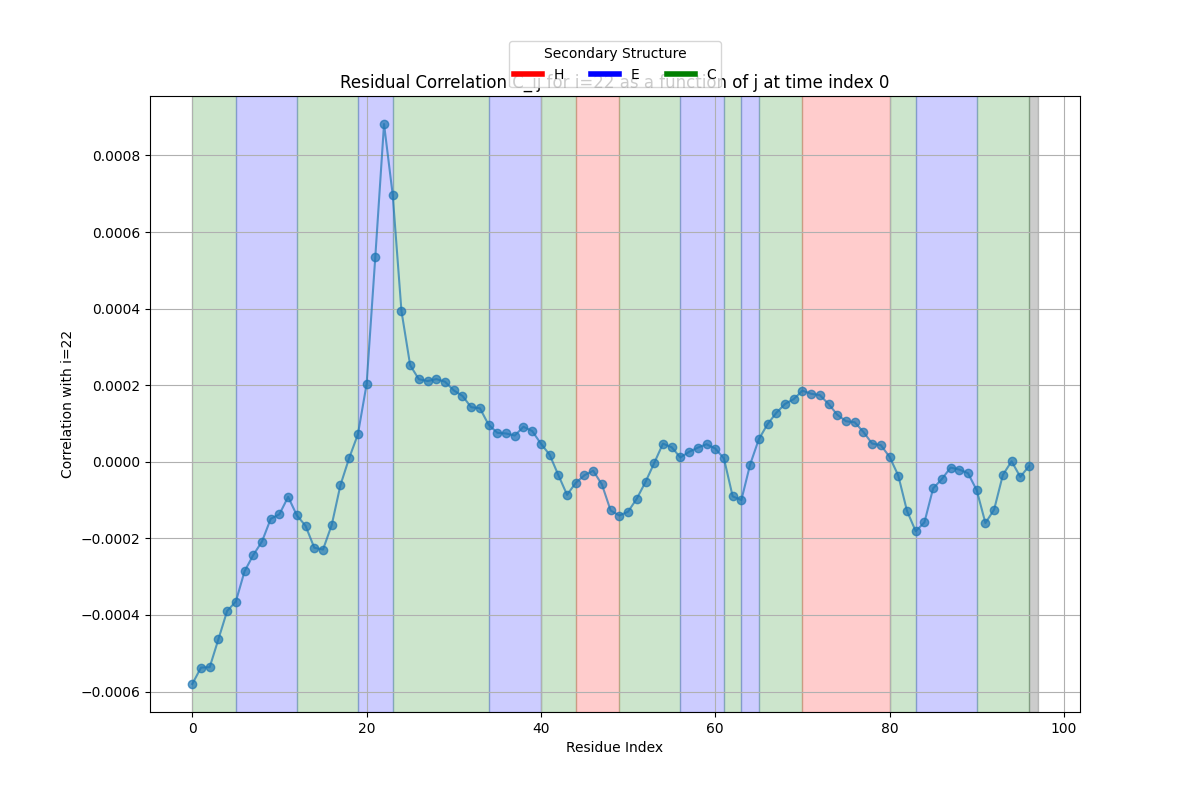
\includegraphics[width=0.5\textwidth]{images/2m0zResidual Correlation C_ij for i=22 as a function of j at time index 0.png}
    \caption{Correlazione}
\end{figure}
\begin{figure}[H]
    \centering
    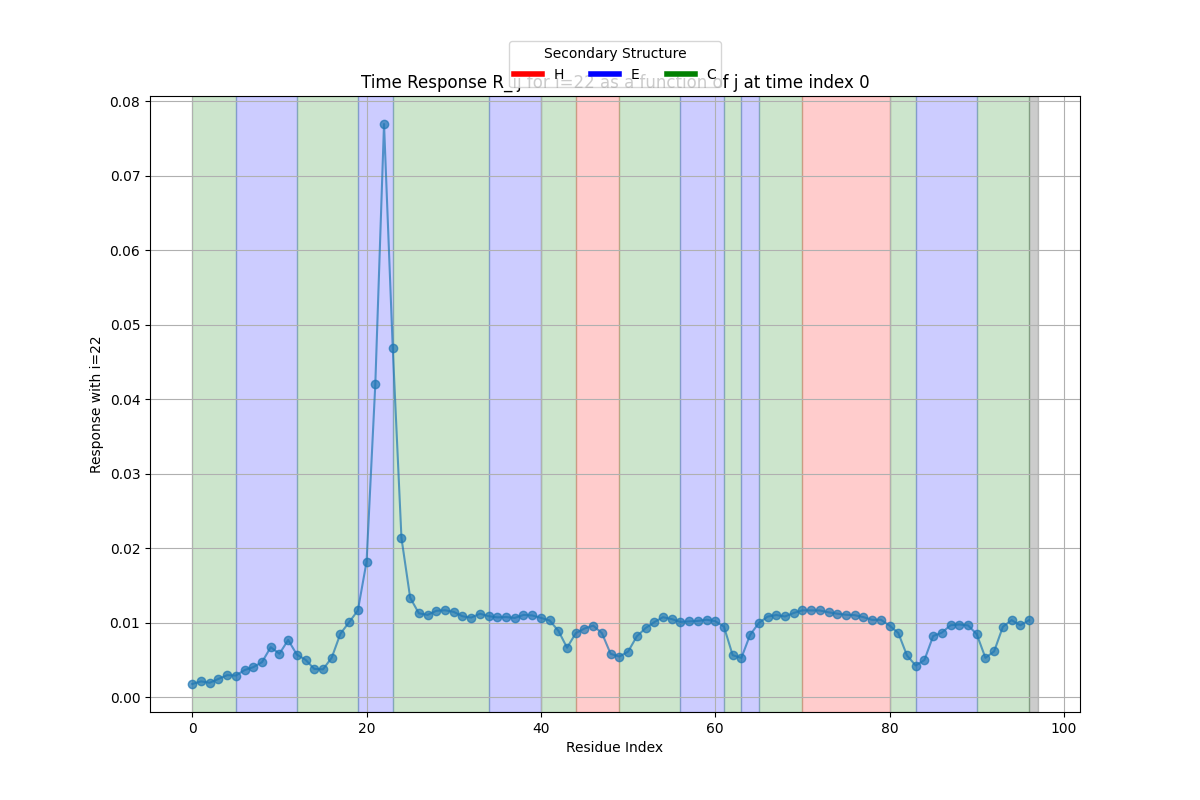
\includegraphics[width=0.5\textwidth]{"images/2m0zTime Response R_ij for i=22 as a function of j at time index 0.png"}
    \caption{Risposta}
\end{figure}

\begin{figure}[H]
    \centering
    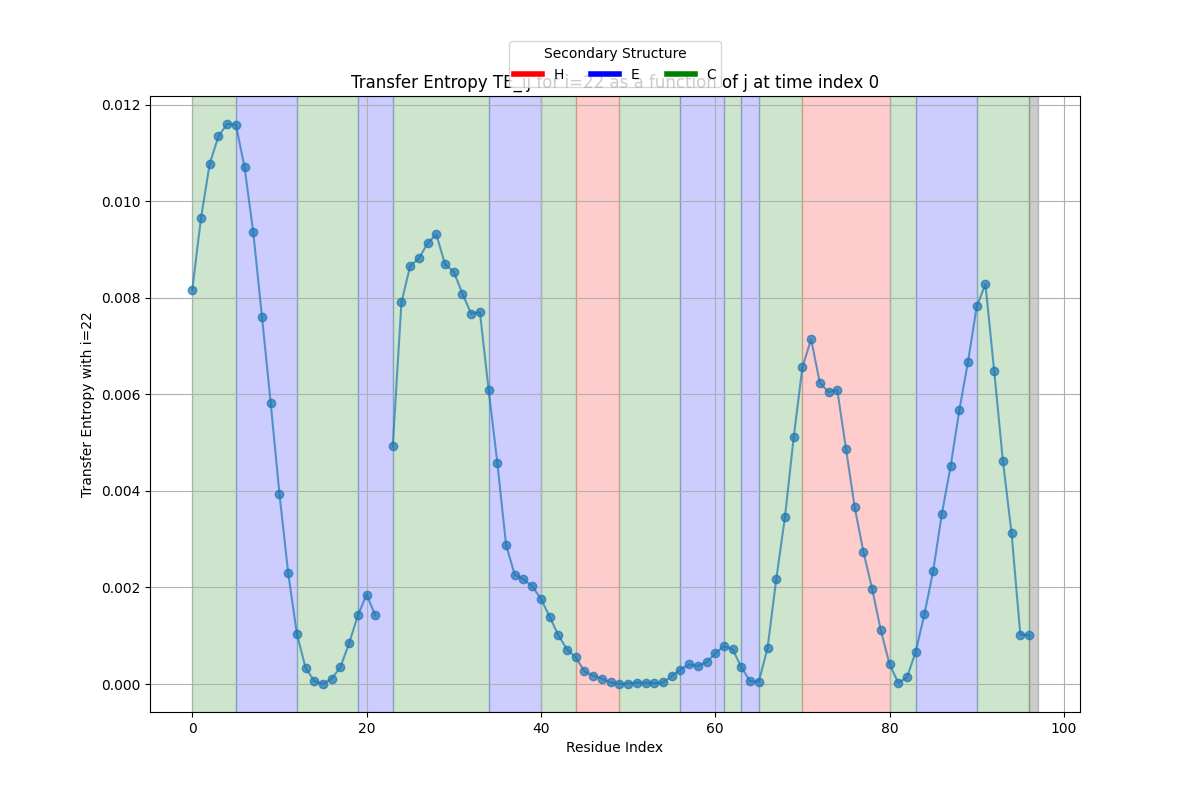
\includegraphics[width=0.5\textwidth]{"images/2m0zTransfer Entropy TE_ij for i=22 as a function of j at time index 0.png"}
    \caption{Transfer Entropy}
\end{figure}
\begin{figure}[H]
    \centering
    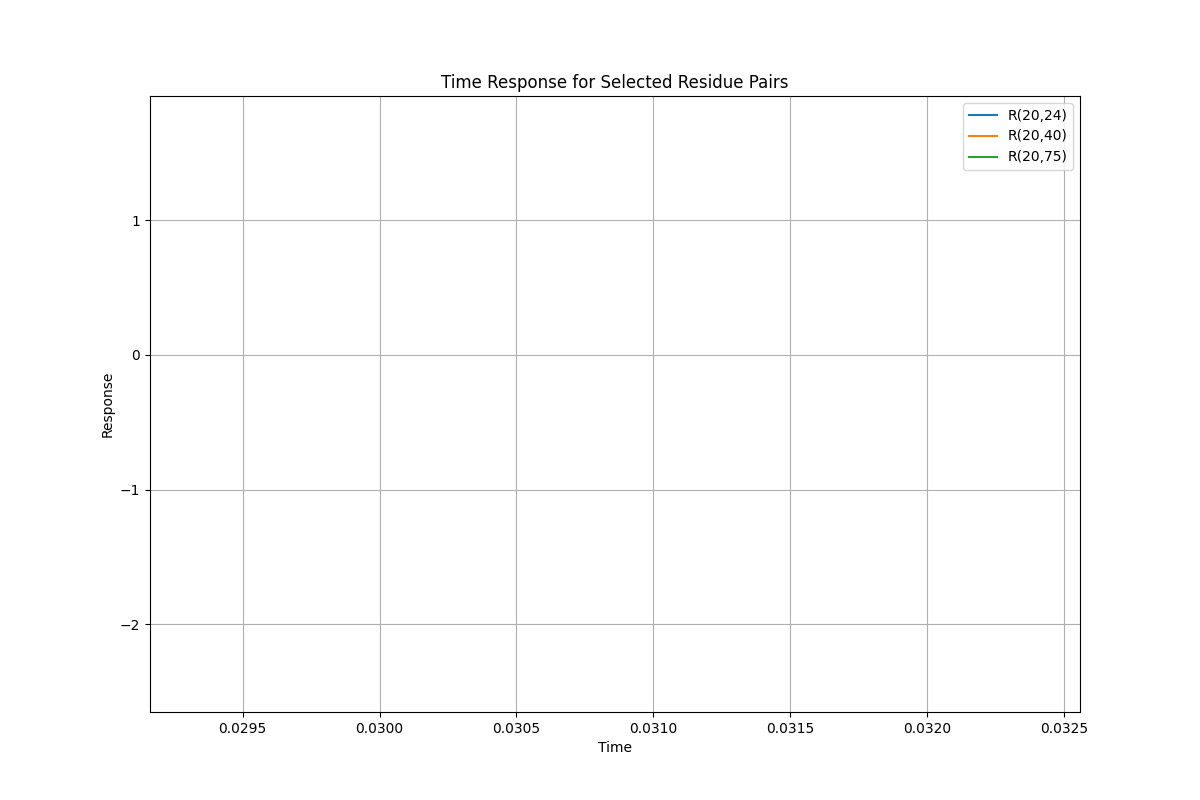
\includegraphics[width=0.5\textwidth]{"images/2m0zMultiple_time_resposne.png"}
    \caption{Multiple time response}
\end{figure}

\begin{figure}[H]
    \centering
    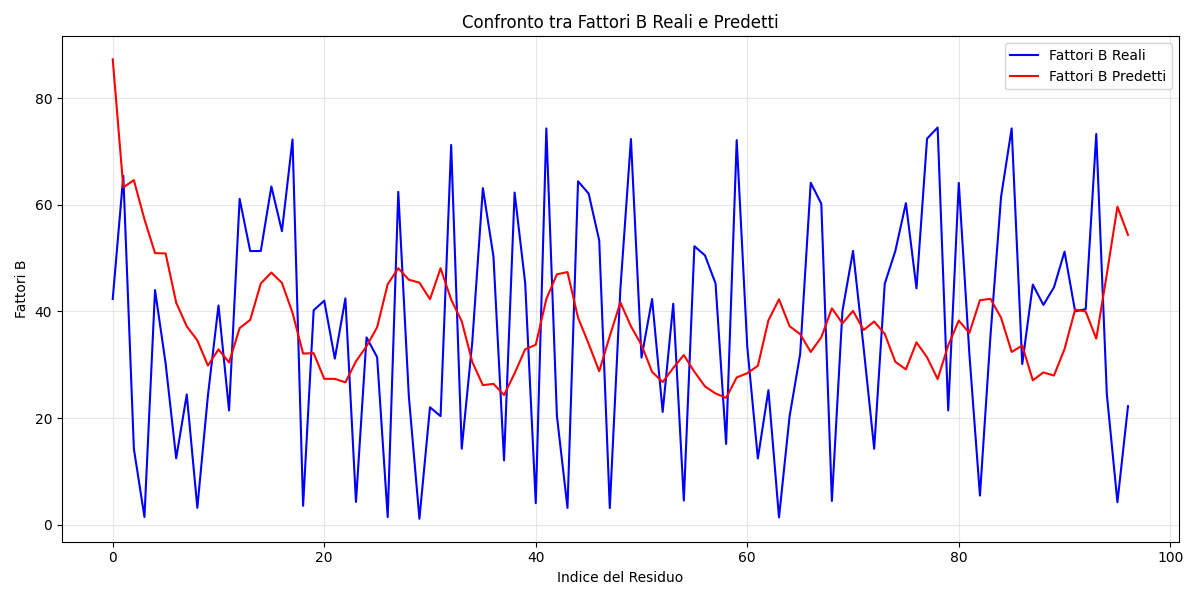
\includegraphics[width=0.5\textwidth]{"images/2m0zConfronto tra Fattori B Reali e Predetti.png"}
    \caption{B factors}
\end{figure}
\begin{figure}[H]
    \centering
    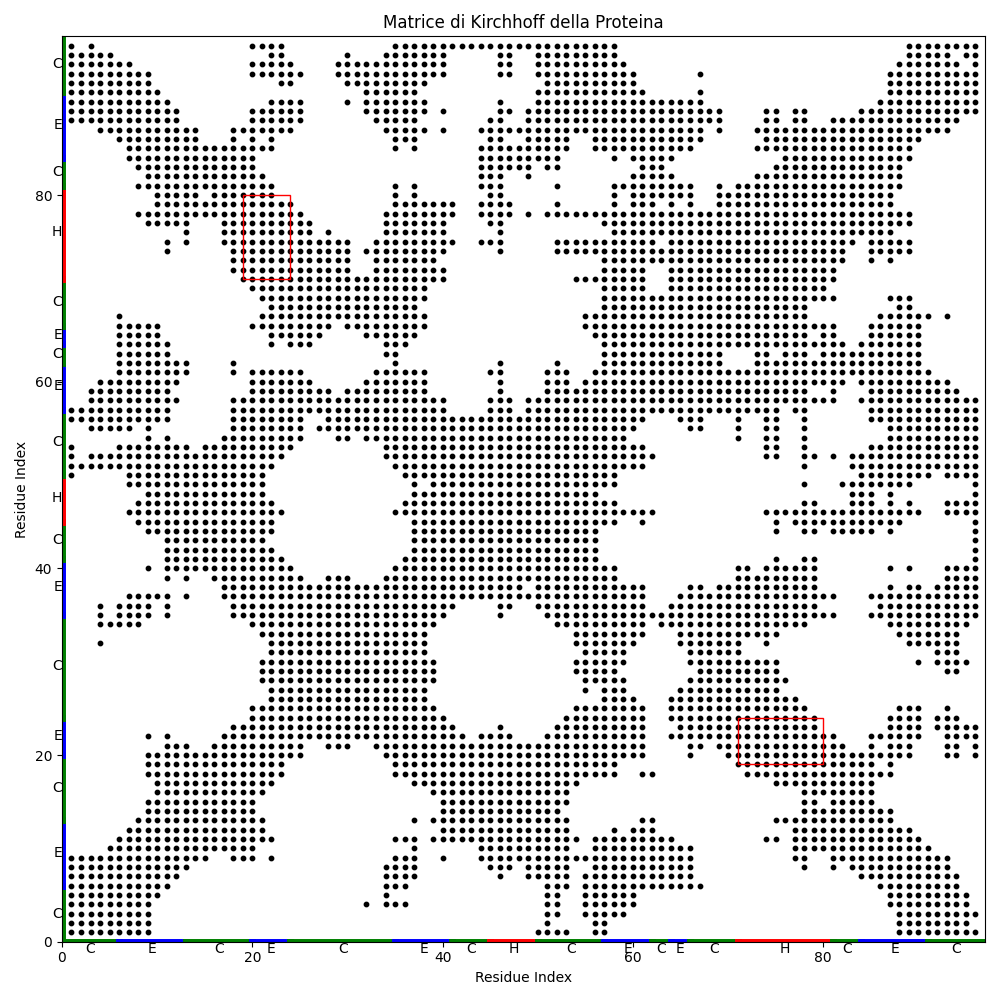
\includegraphics[width=0.5\textwidth]{"images/2m0z_Matrice di Kirchhoff della Proteina.png"}
    \caption{Kirchhoff}
\end{figure}
\begin{figure}[H]
    \centering
    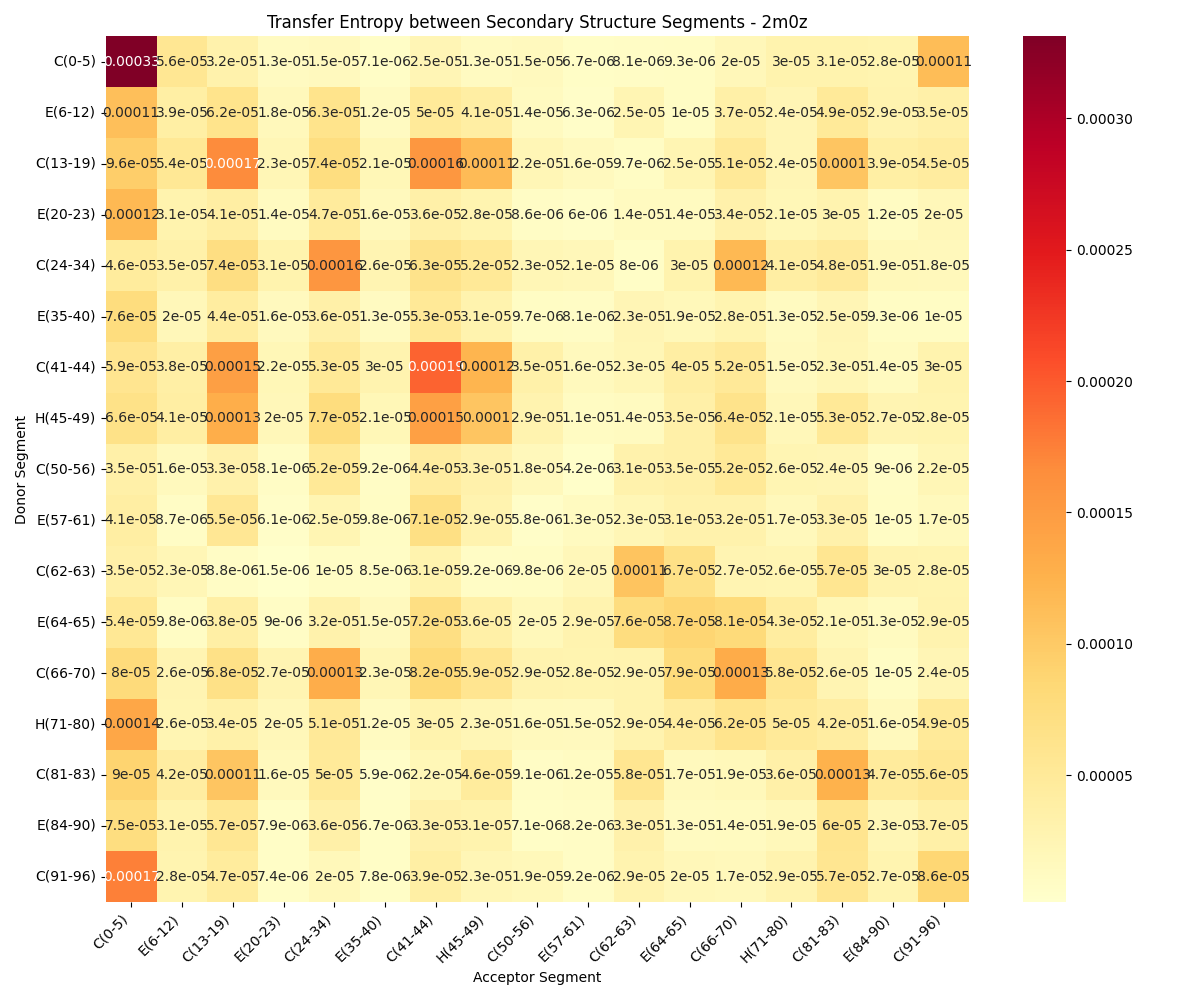
\includegraphics[width=0.5\textwidth]{"images/2m0zanalyze_secondary_structure_transfer_entropy.png"}
    \caption{Secodnaria Structure}
\end{figure}
\section{2M10}
\begin{figure}[H]
    \centering                            
    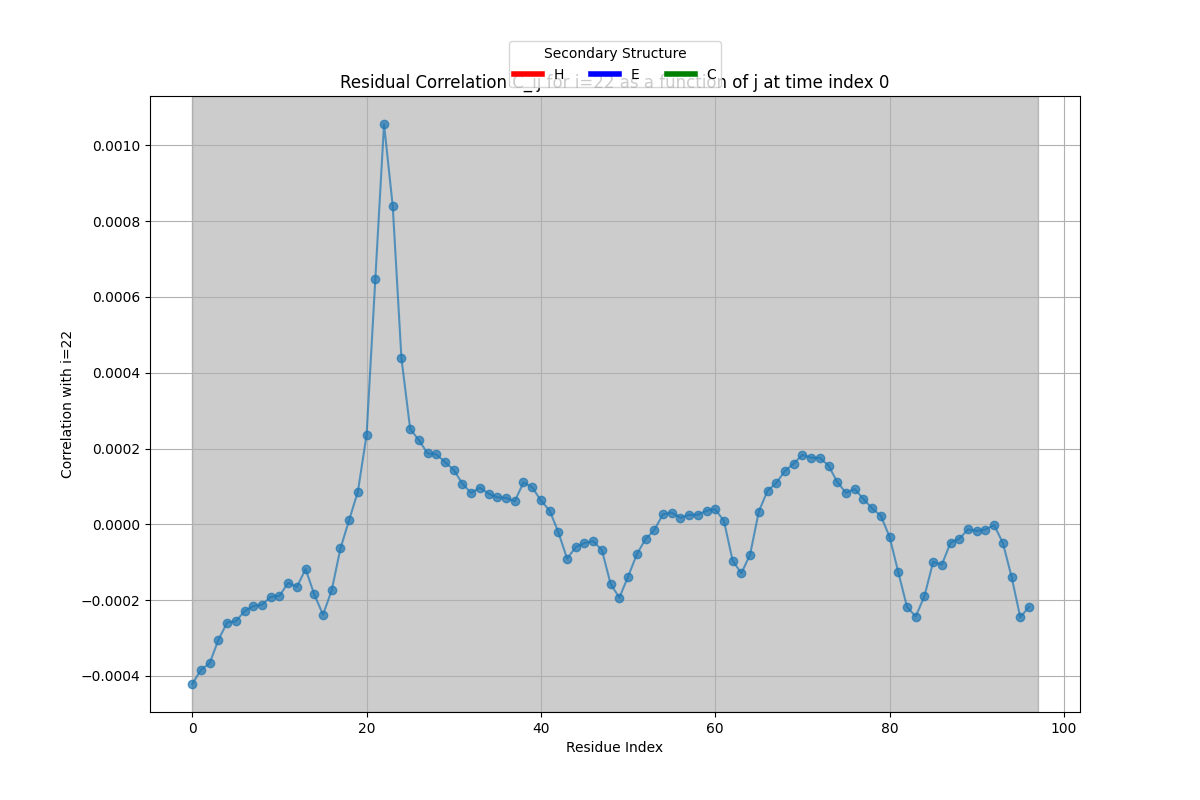
\includegraphics[width=0.5\textwidth]{"images/2m10Residual Correlation C_ij for i=22 as a function of j at time index 0.png"}
    \caption{Correlazione}
\end{figure}
\begin{figure}[H]
    \centering
    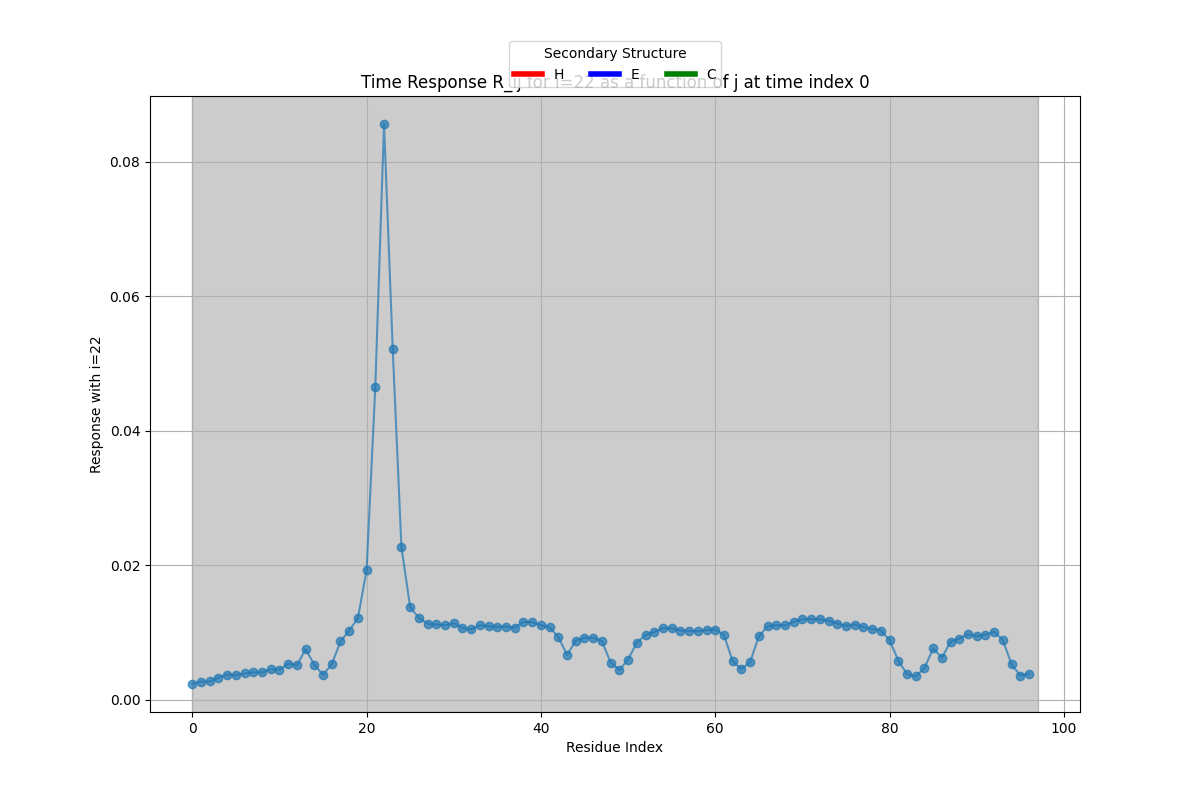
\includegraphics[width=0.5\textwidth]{"images/2m10Time Response R_ij for i=22 as a function of j at time index 0.png"}
    \caption{Risposta}
\end{figure}

\begin{figure}[H]
    \centering
    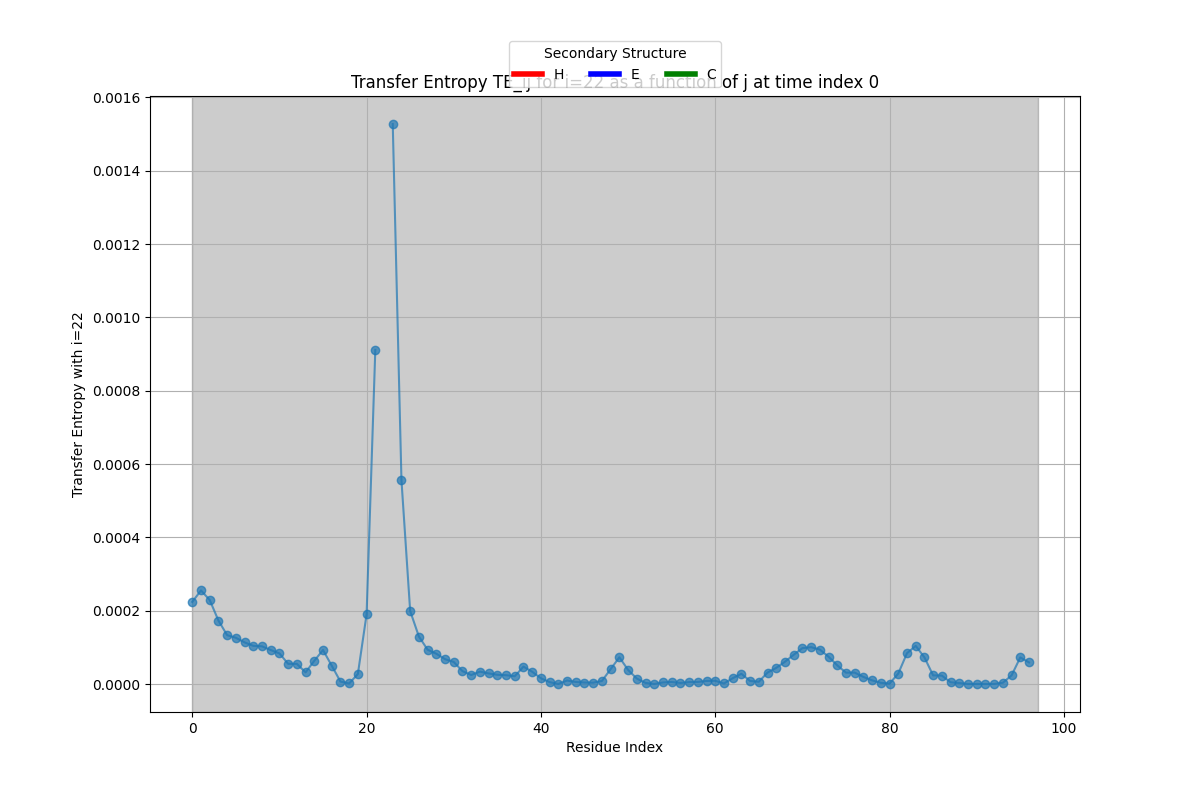
\includegraphics[width=0.5\textwidth]{"images/2m10Transfer Entropy TE_ij for i=22 as a function of j at time index 0.png"}
    \caption{Transfer Entropy}
\end{figure}
\begin{figure}[H]
    \centering
    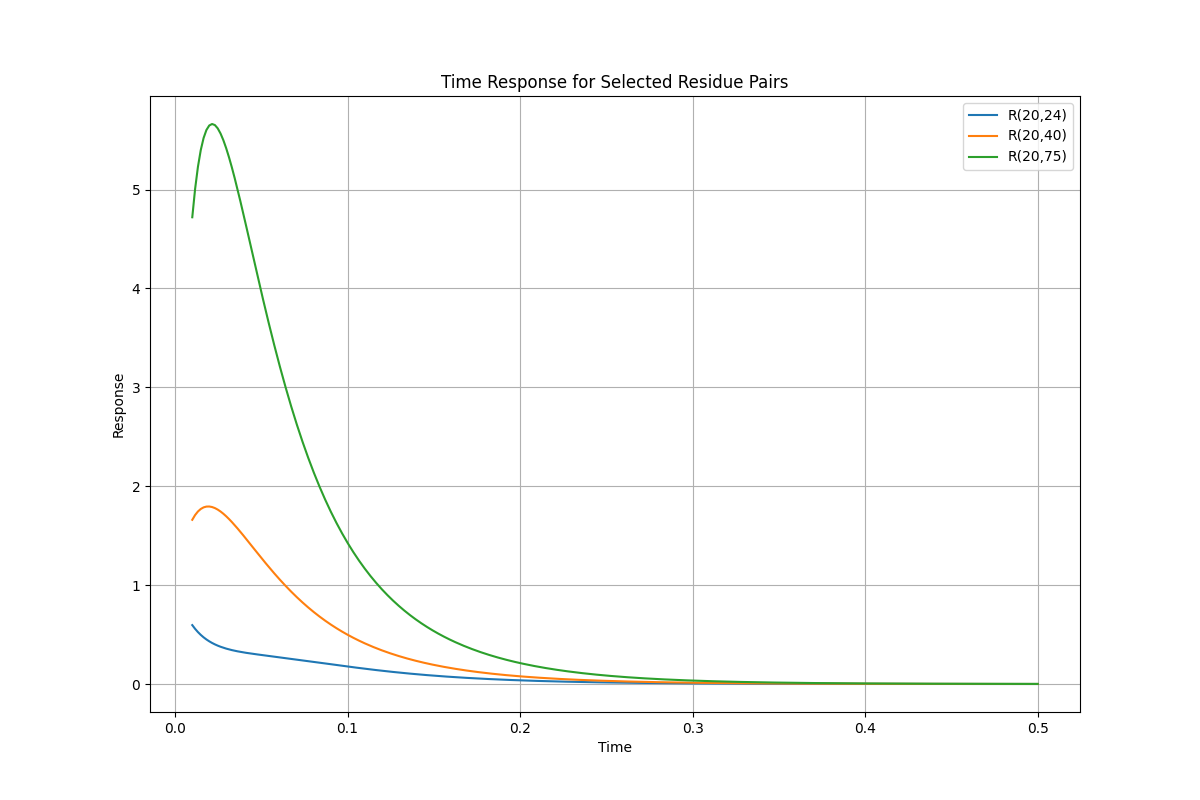
\includegraphics[width=0.5\textwidth]{"images/2m10Multiple_time_resposne.png"}
    \caption{Multiple time response}
\end{figure}

\begin{figure}[H]
    \centering
    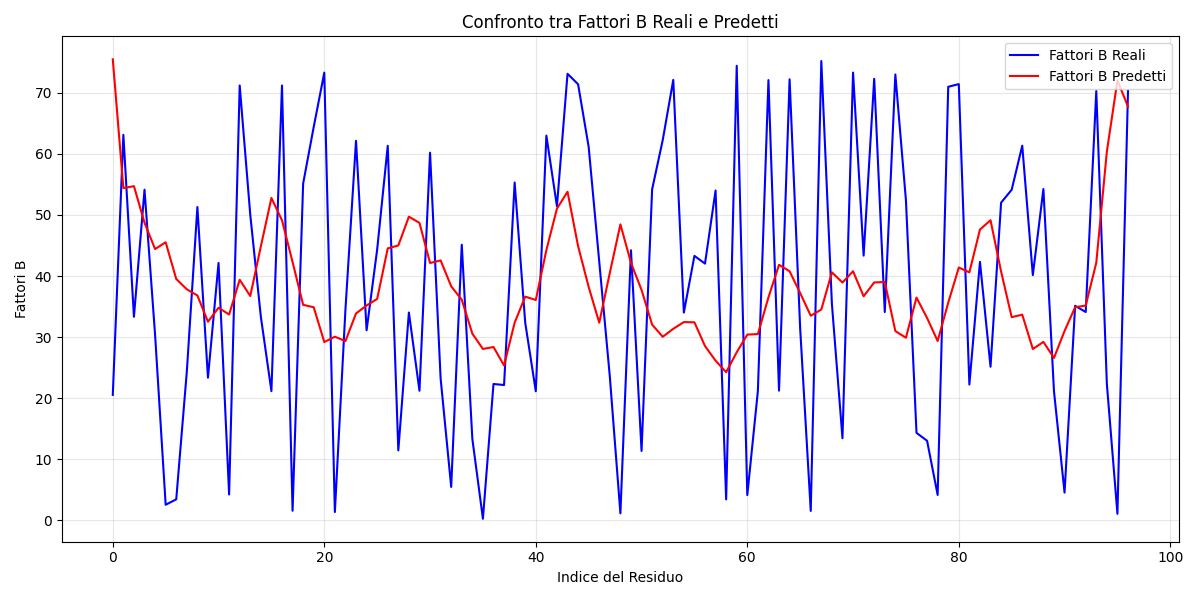
\includegraphics[width=0.5\textwidth]{"images/2m10Confronto tra Fattori B Reali e Predetti.png"}
    \caption{B factors}
\end{figure}
\begin{figure}[H]
    \centering
    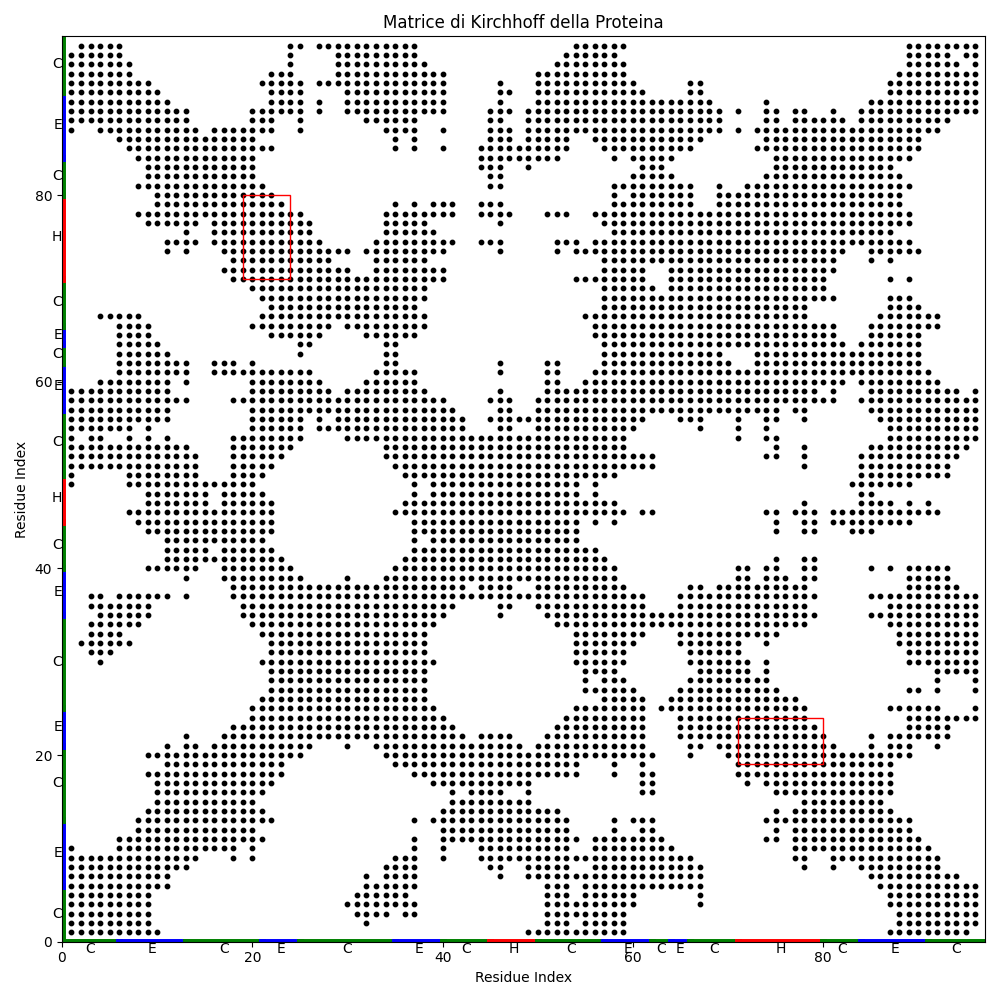
\includegraphics[width=0.5\textwidth]{"images/2m10_Matrice di Kirchhoff della Proteina.png"}
    \caption{Kirchhoff}
\end{figure}
\begin{figure}[H]
    \centering
    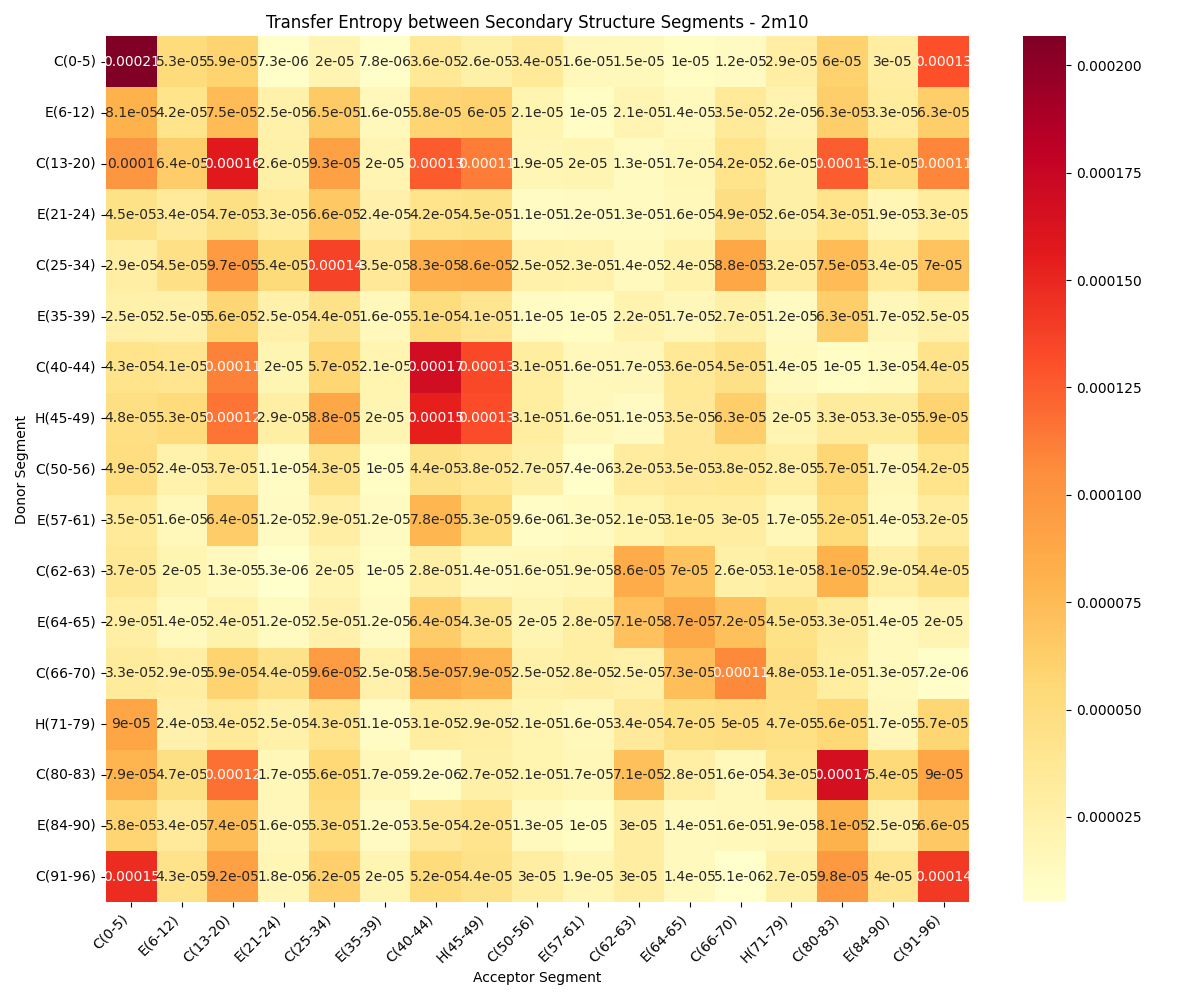
\includegraphics[width=0.5\textwidth]{"images/2m10analyze_secondary_structure_transfer_entropy.png"}
    \caption{Transfer struttura Secondaria}
\end{figure}
\section{3LNX}
\begin{figure}[H]
    \centering
    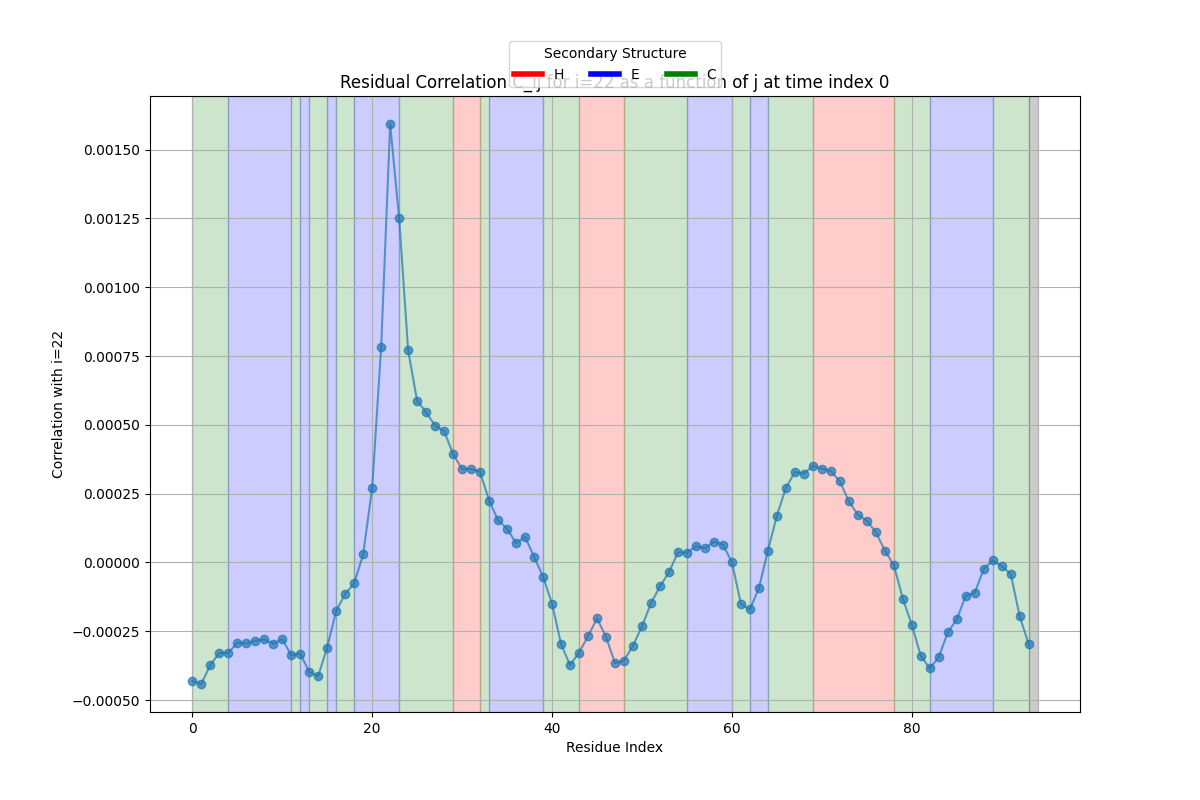
\includegraphics[width=0.5\textwidth]{"images/3LNXResidual Correlation C_ij for i=22 as a function of j at time index 0.png"}
    \caption{Correlazione}
\end{figure}
\begin{figure}[H]
    \centering
    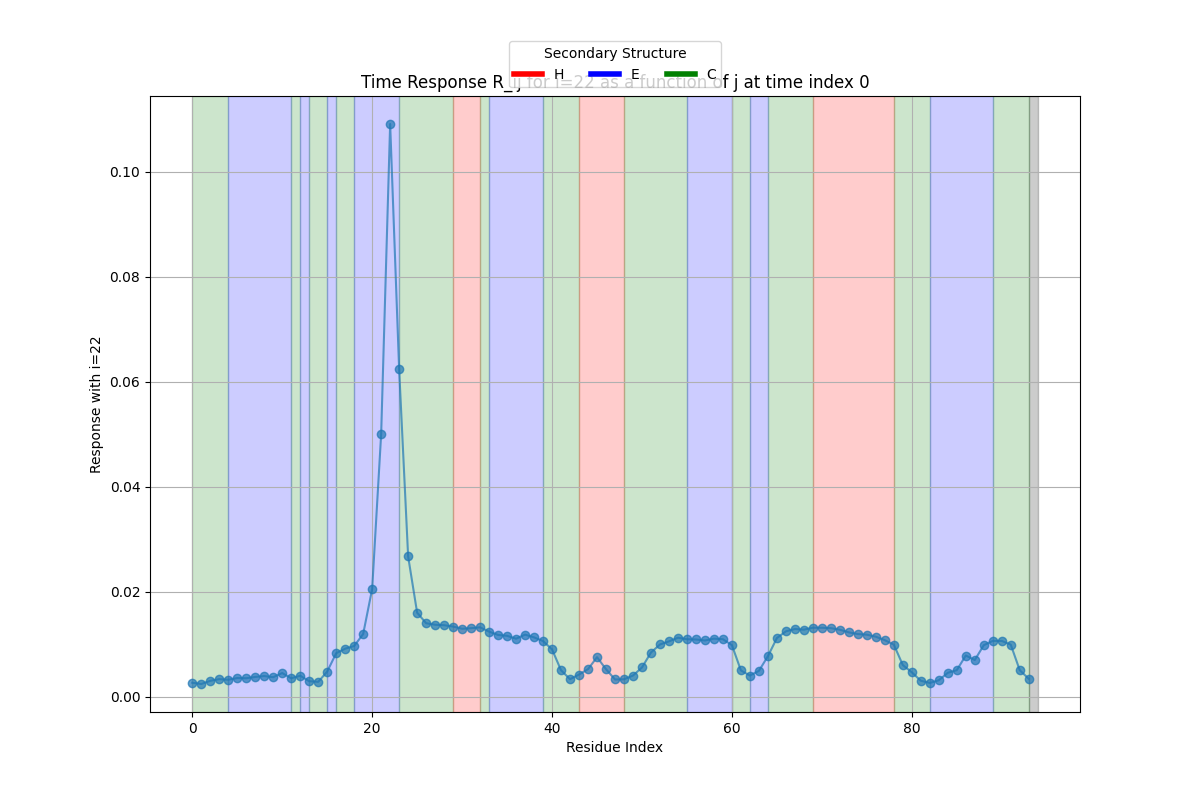
\includegraphics[width=0.5\textwidth]{"images/3LNXTime Response R_ij for i=22 as a function of j at time index 0.png"}
    \caption{Risposta}
\end{figure}

\begin{figure}[H]
    \centering
    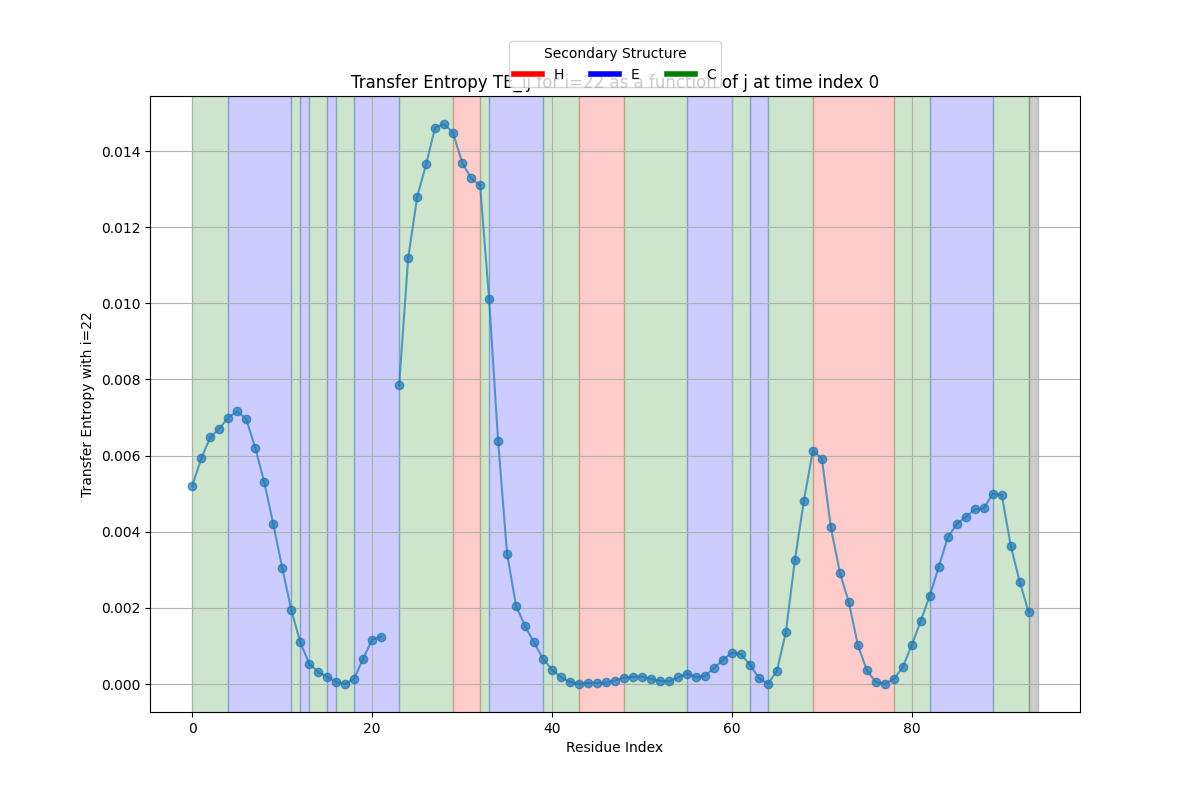
\includegraphics[width=0.5\textwidth]{"images/3LNXTransfer Entropy TE_ij for i=22 as a function of j at time index 0.png"}
    \caption{Transfer Entropy}
\end{figure}
\begin{figure}[H]
    \centering
    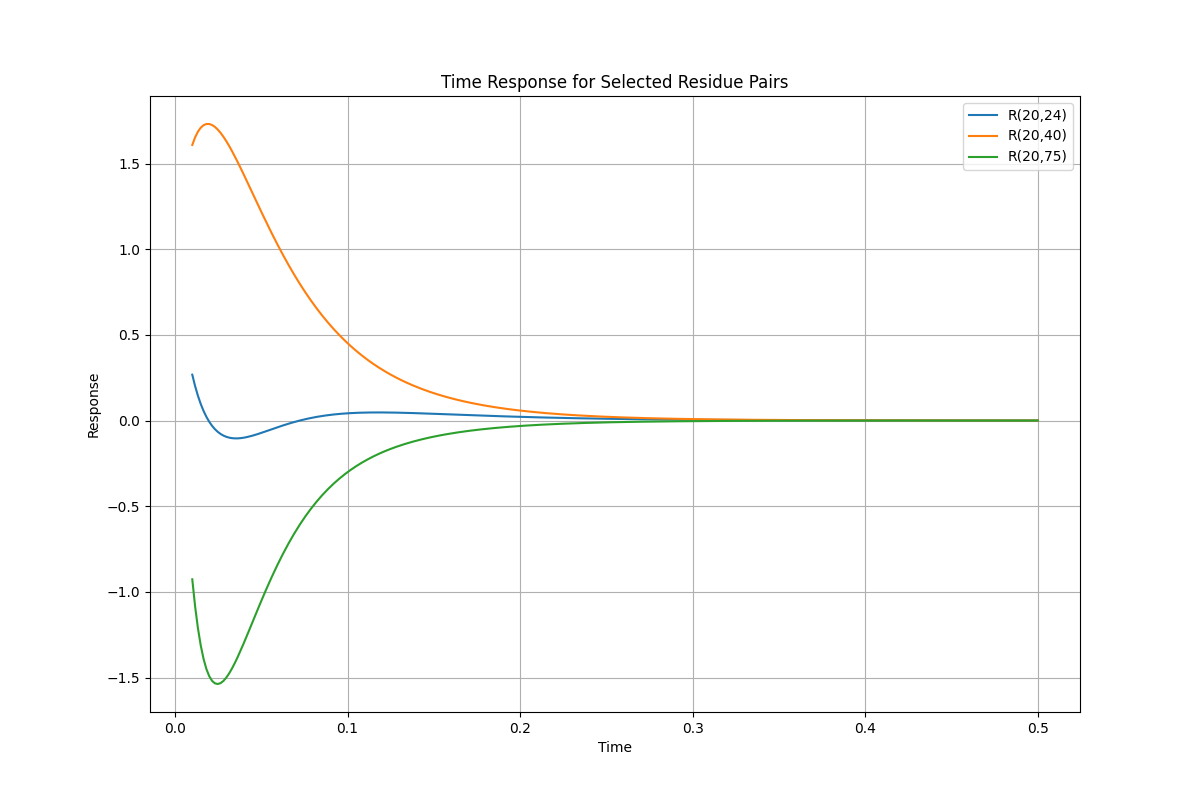
\includegraphics[width=0.5\textwidth]{"images/3LNXMultiple_time_resposne.png"}
    \caption{Multiple time response}
\end{figure}

\begin{figure}[H]
    \centering
    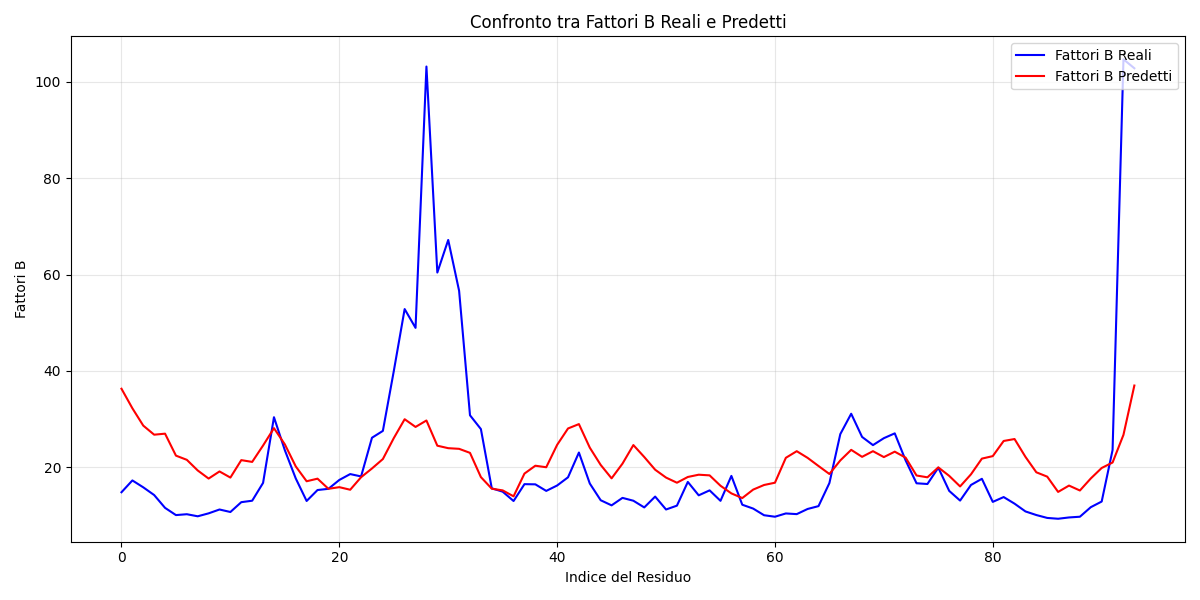
\includegraphics[width=0.5\textwidth]{"images/3LNXConfronto tra Fattori B Reali e Predetti.png"}
    \caption{B factors}
\end{figure}
\begin{figure}[H]
    \centering
    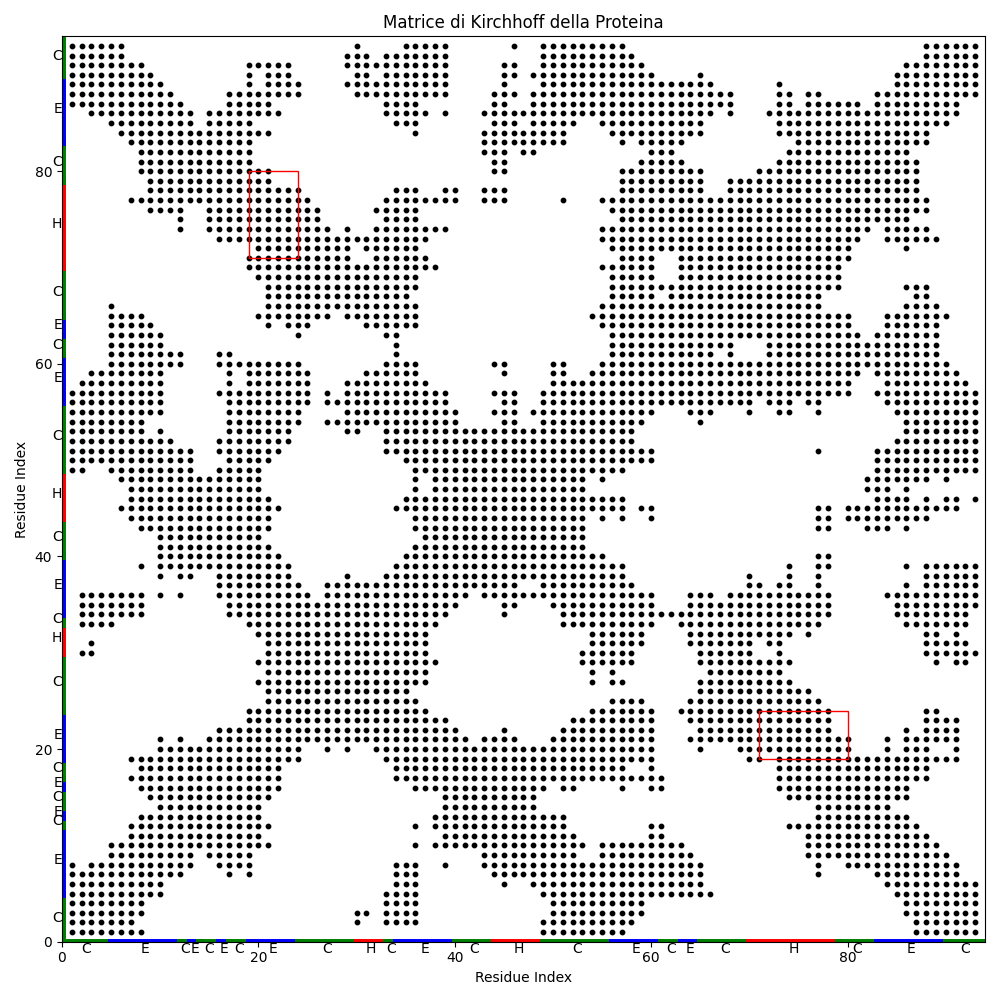
\includegraphics[width=0.5\textwidth]{"images/3LNX_Matrice di Kirchhoff della Proteina.png"}
    \caption{Kirchhoff}
\end{figure}
\begin{figure}[H]
    \centering
    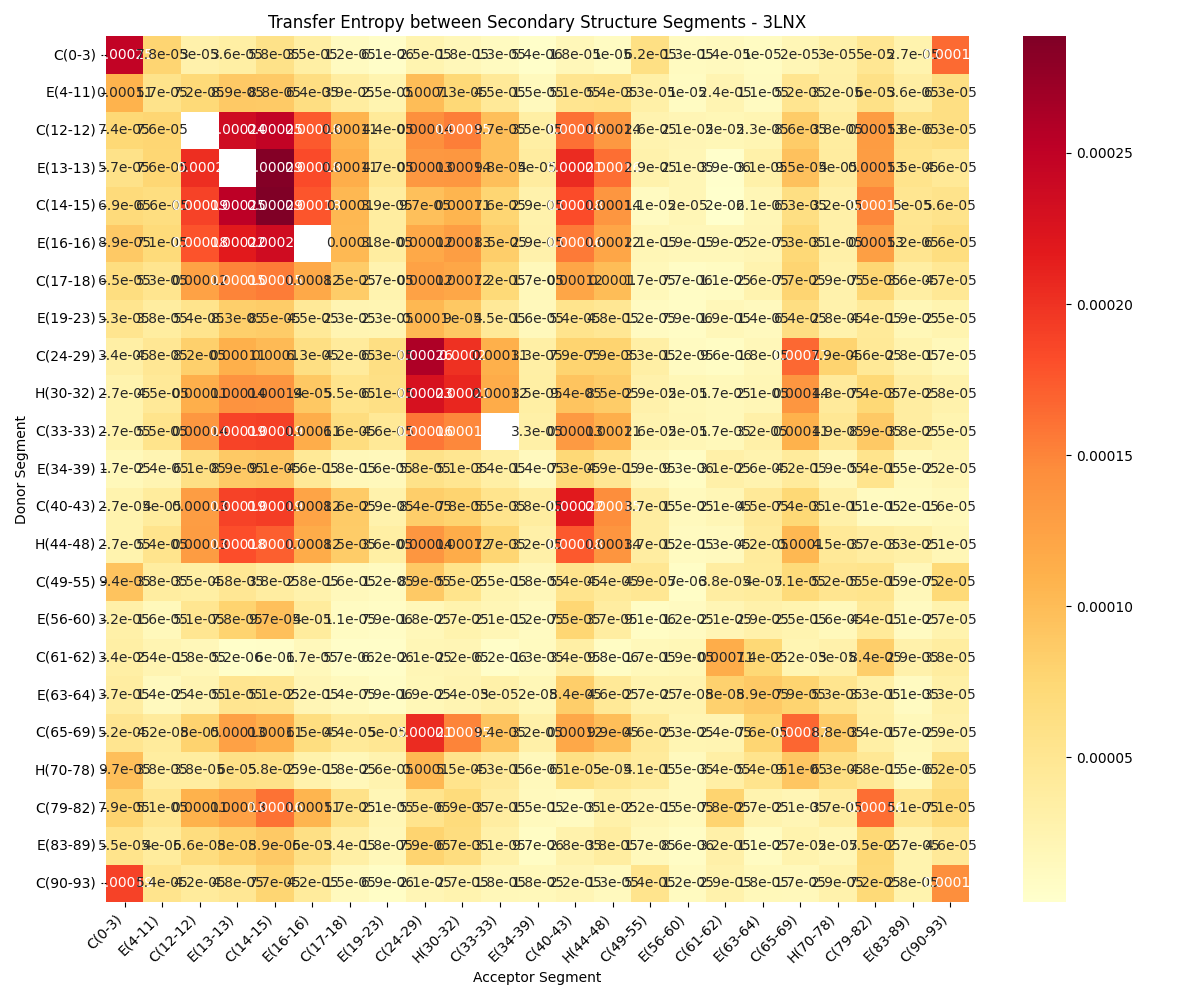
\includegraphics[width=0.5\textwidth]{"images/3LNXanalyze_secondary_structure_transfer_entropy.png"}
    \caption{Secondaria}
\end{figure}
\section{3LNY}
\begin{figure}[H]
    \centering
    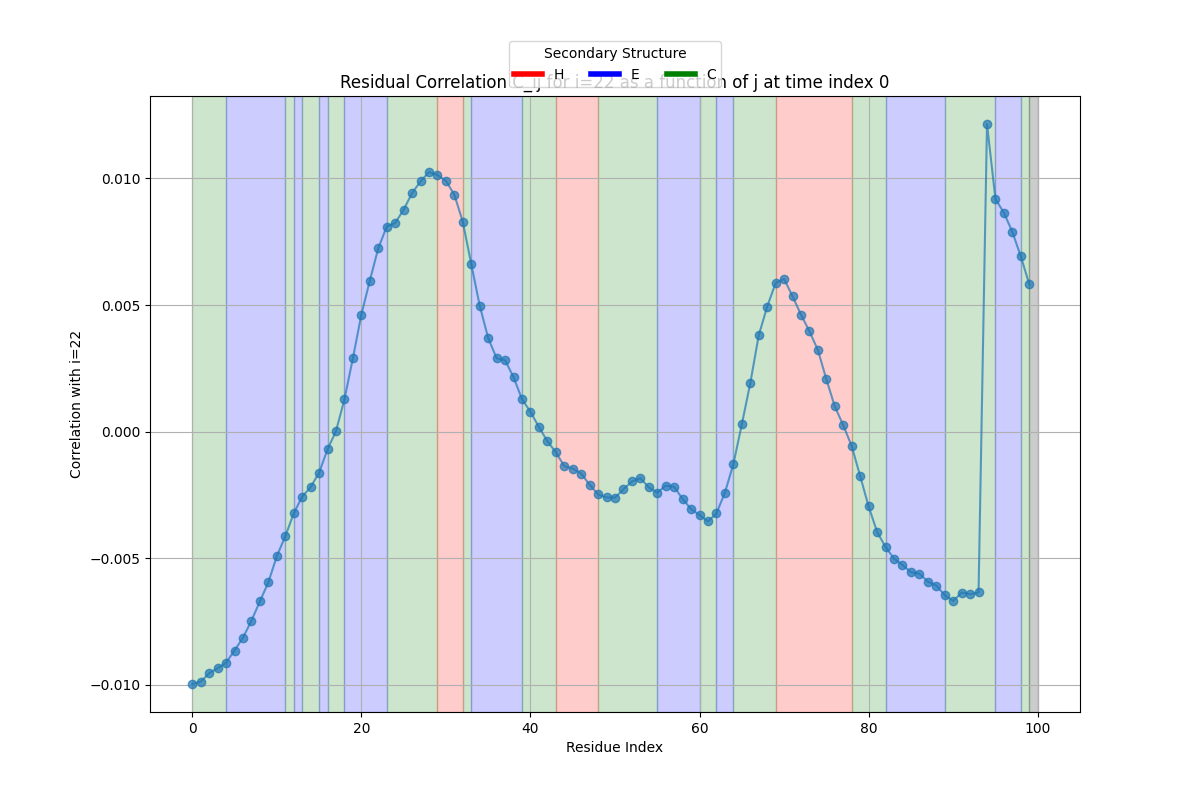
\includegraphics[width=0.5\textwidth]{"images/3LNYResidual Correlation C_ij for i=22 as a function of j at time index 0.png"}
    \caption{Correlazione}
\end{figure}
\begin{figure}[H]
    \centering
    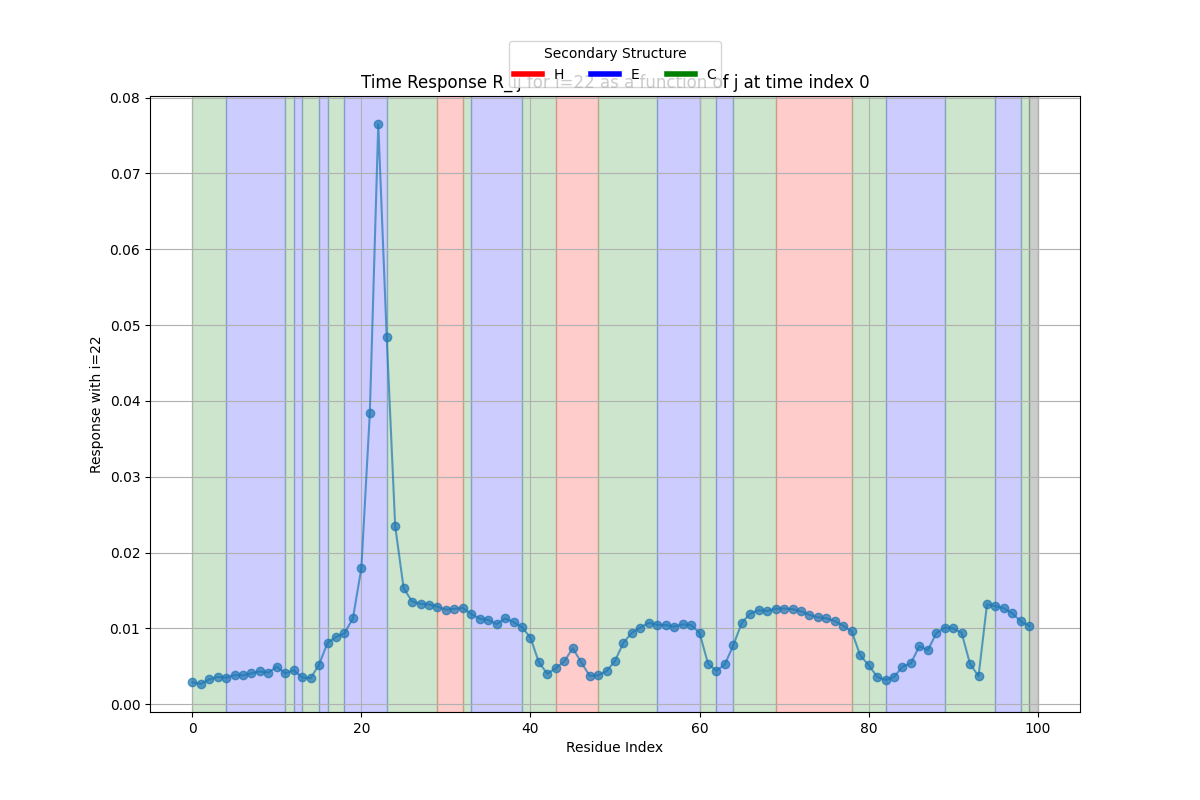
\includegraphics[width=0.5\textwidth]{"images/3LNYTime Response R_ij for i=22 as a function of j at time index 0.png"}
    \caption{Risposta}
\end{figure}

\begin{figure}[H]
    \centering
    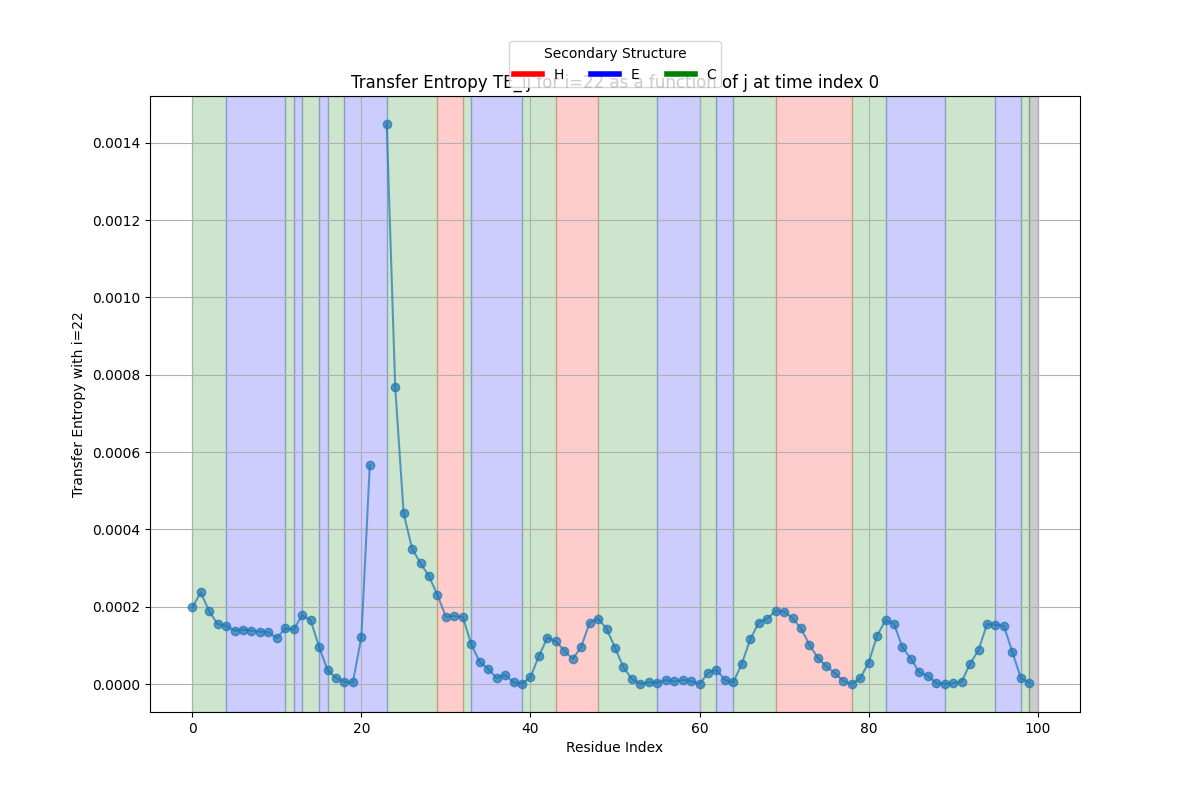
\includegraphics[width=0.5\textwidth]{"images/3LNYTransfer Entropy TE_ij for i=22 as a function of j at time index 0.png"}
    \caption{Transfer Entropy}
\end{figure}


\begin{figure}[H]
    \centering
    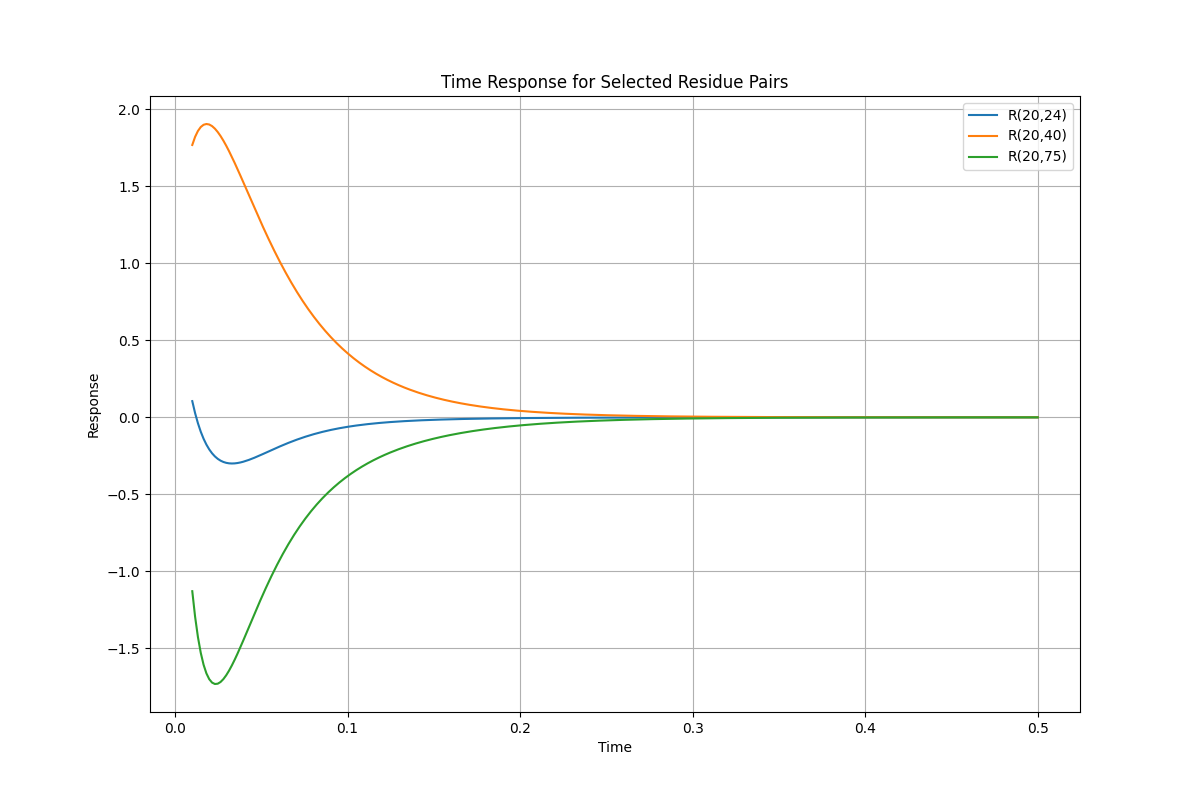
\includegraphics[width=0.5\textwidth]{"images/3LNYMultiple_time_resposne.png"}
    \caption{Multiple time response}
\end{figure}

\begin{figure}[H]
    \centering
    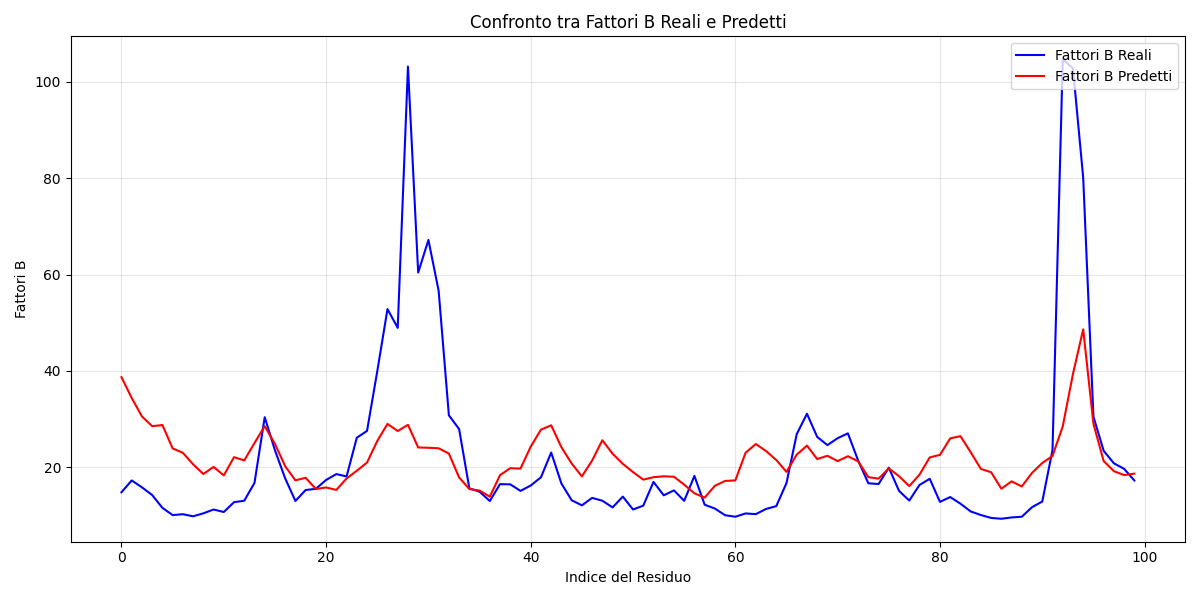
\includegraphics[width=0.5\textwidth]{"images/3LNYConfronto tra Fattori B Reali e Predetti.png"}
    \caption{B factors}
\end{figure}
\begin{figure}[H]
    \centering
    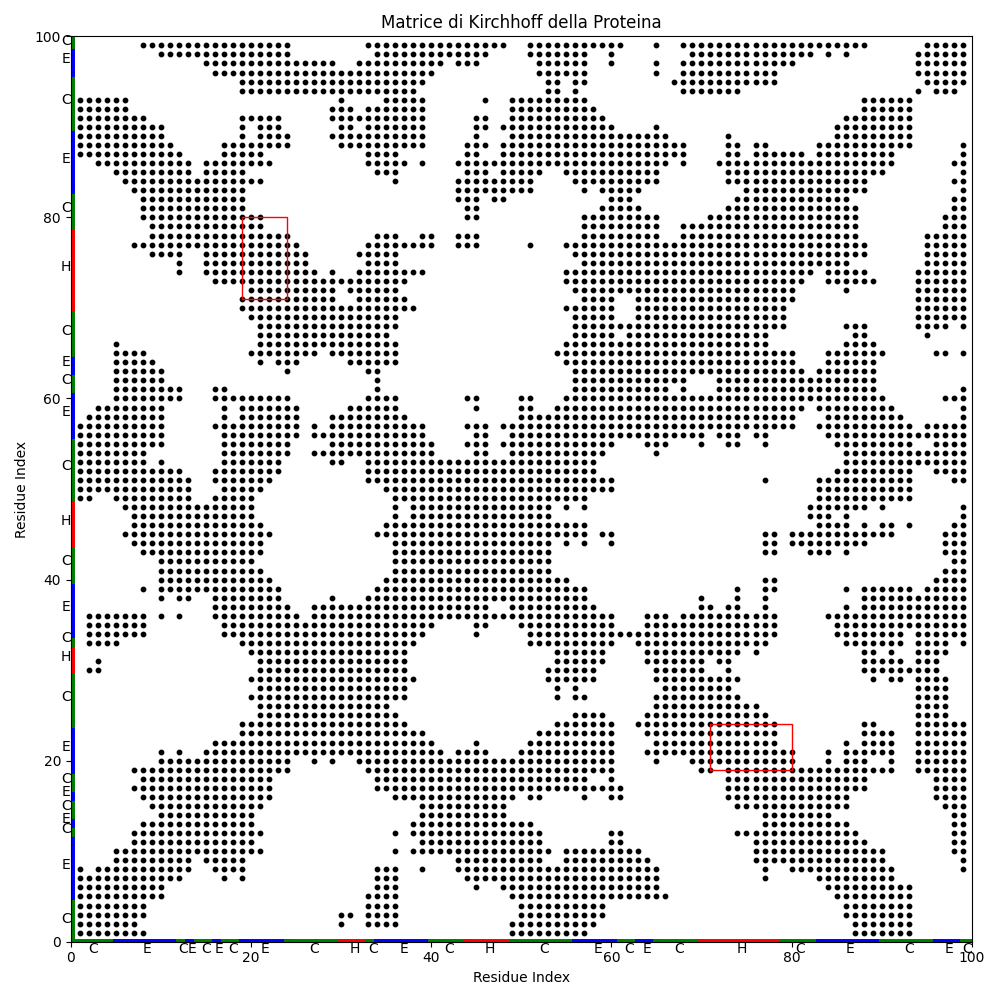
\includegraphics[width=0.5\textwidth]{"images/3LNY_Matrice di Kirchhoff della Proteina.png"}
    \caption{Kirchhoff}
\end{figure}
\begin{figure}[H]
    \centering
    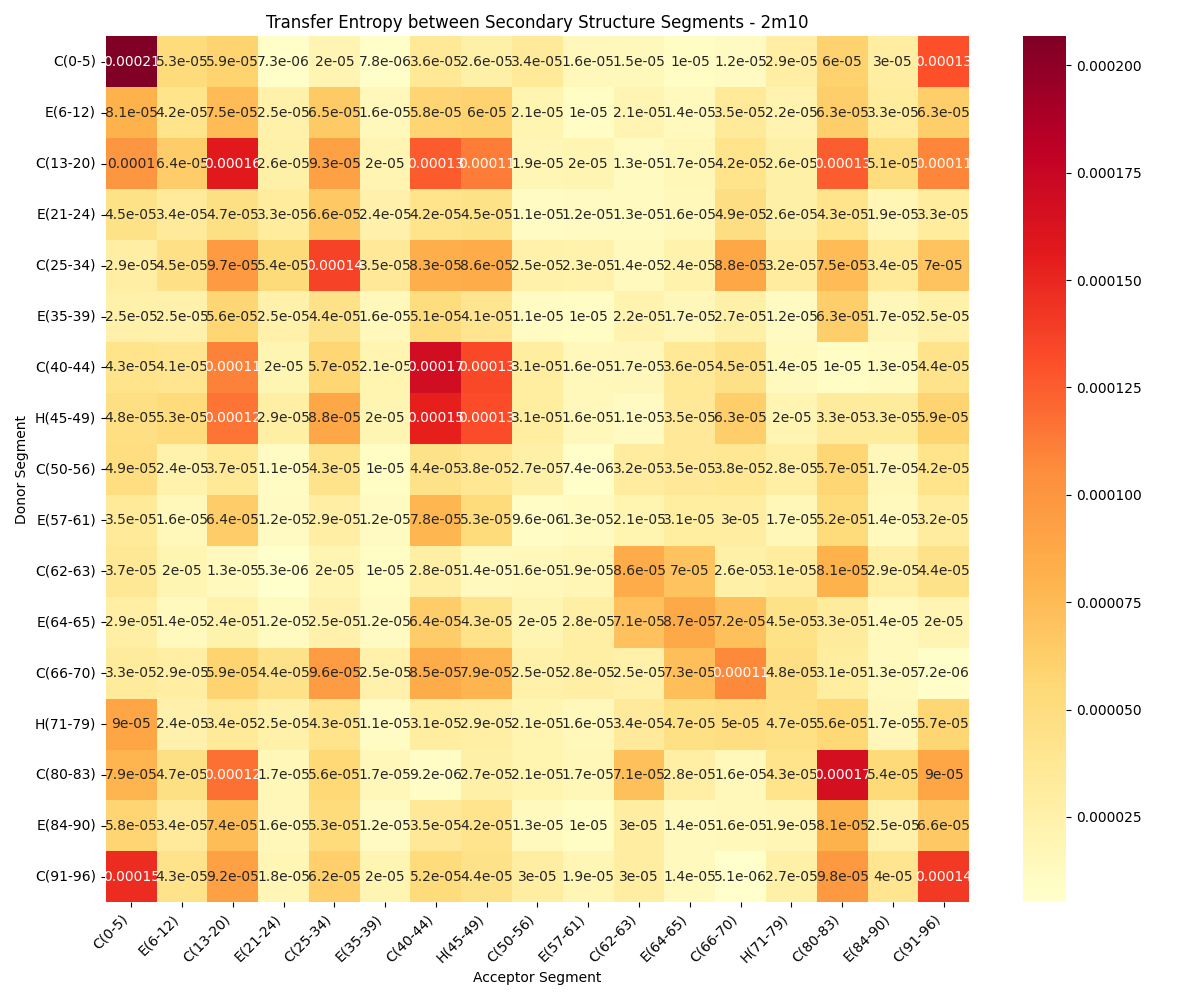
\includegraphics[width=0.5\textwidth]{"images/2m10analyze_secondary_structure_transfer_entropy.png"}
    \caption{Seocndaria}
\end{figure}
\section{Dinamica}
\begin{equation}
    \gamma \dot{x}_i = -g \sum_j K_{ij} x_j + \epsilon(t) (r_{21} - r_{76}) \delta_{i,21} - \epsilon(t) (r_{21} - r_{76}) \delta_{i,76} + \sqrt{2 \gamma k_B T} \xi_i(t)
    \end{equation}
Ora posso simulare il moto Time dependent di ogni atomo e vedere come si propagano le vibrazioni.
Gli autovalori sono smere le frequeze naturali del sistema.
\begin{figure}[H]
    \centering
    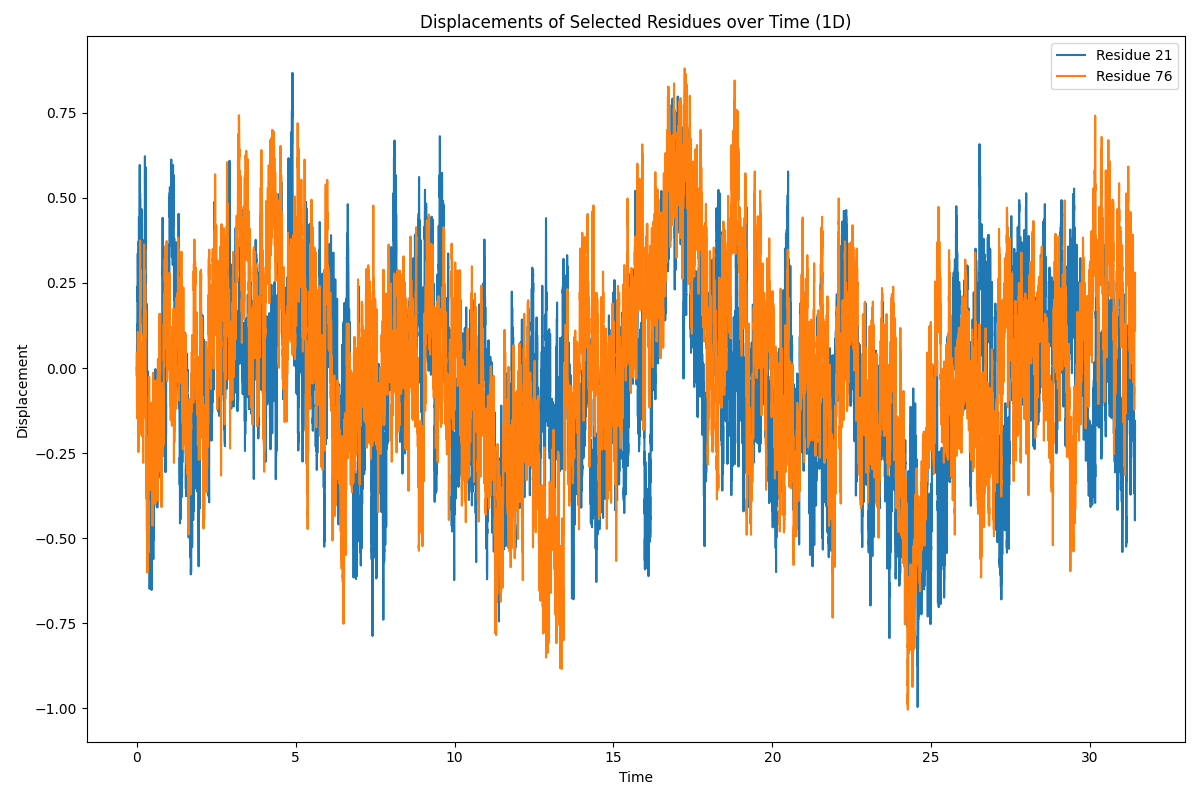
\includegraphics[width=0.5\textwidth]{"images/2m10_Processo_stocastico.png"}
    \caption{Seocndaria}
\end{figure}
\begin{figure}[H]
    \centering
    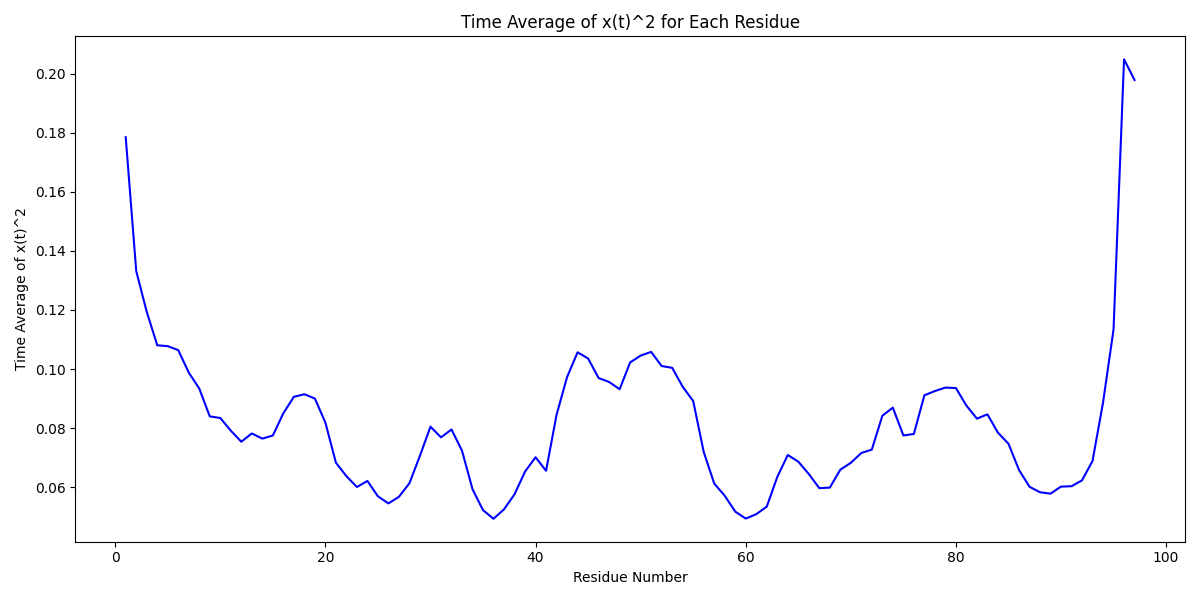
\includegraphics[width=0.5\textwidth]{"images/2m10_Stima beta factors.png"}
    \caption{Seocndaria}
\end{figure}
\section{Gradienete di temperature}
\begin{equation}
    \boldsymbol{\gamma}_i \dot{x}_i = -g \sum_j K_{ij} x_j  + \sqrt{2 \boldsymbol{\gamma}_i k_B \boldsymbol{T}_i} \xi_i(t)
    \end{equation}
Gamma e T sono diventati vettori.
Se la risolvi ottieni:
\begin{equation}
    \sum_{u} \exp\left( \sum_j K_{ij} u_j \right) \cdot \beta \cdot \beta^{\top} \cdot \exp\left( \sum_s K_{is} u_s \right)
    \end{equation}
Ora hai diversi modi di scegliere i valori di T:
\section{Troncamento Tmeperatura}
se sono sotto 5 legami allora ho temperatura bassa.
Se sono sopra allora ho temperatura piu' alta.
Posso prendere banalmente 2 valori 0,1 .
\begin{figure}[H]
    \centering
    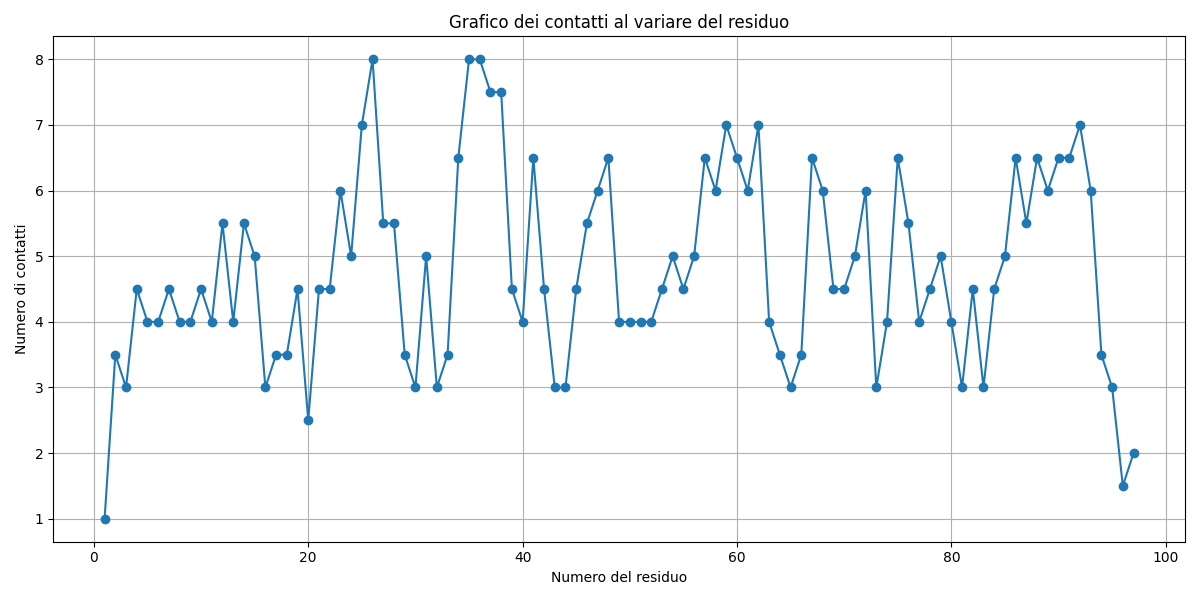
\includegraphics[width=0.5\textwidth]{"images/2m10_2_temperature_contact_cutoff.png"}
    \caption{ Temperatura Troncamento }
\end{figure}
\begin{figure}[H]
    \centering
    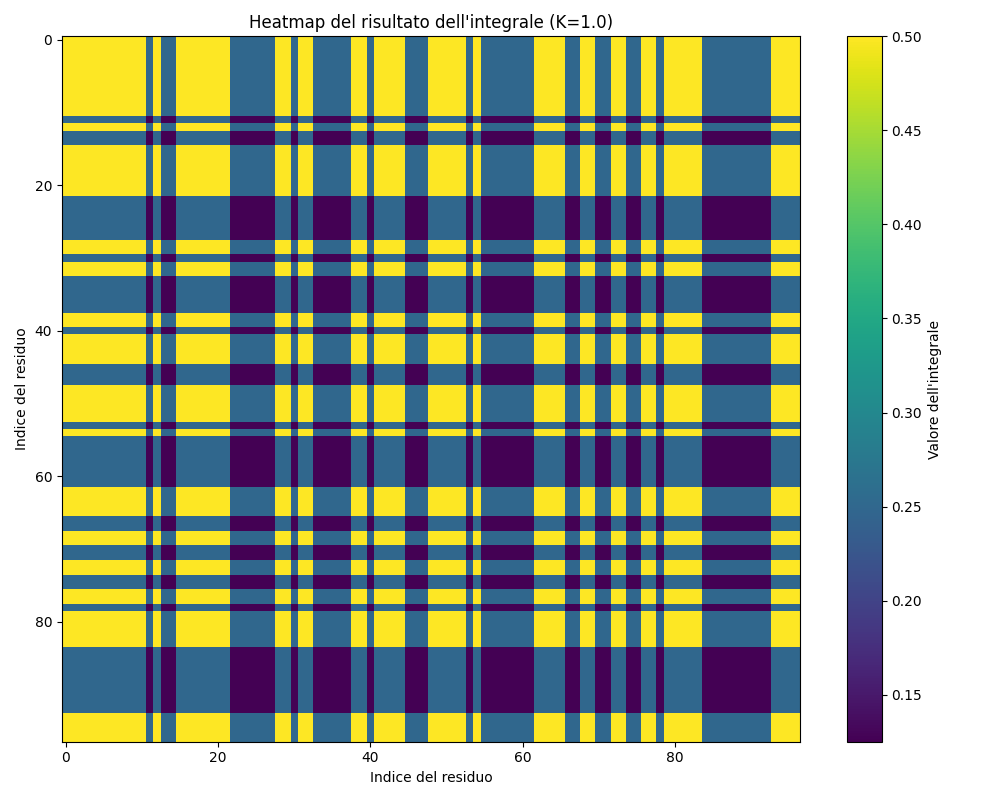
\includegraphics[width=0.5\textwidth]{"images/2m10_2_temperature_correlation_cutoff.png"}
    \caption{ Temperatura Troncamento  }
\end{figure}
\begin{figure}[H]
    \centering
    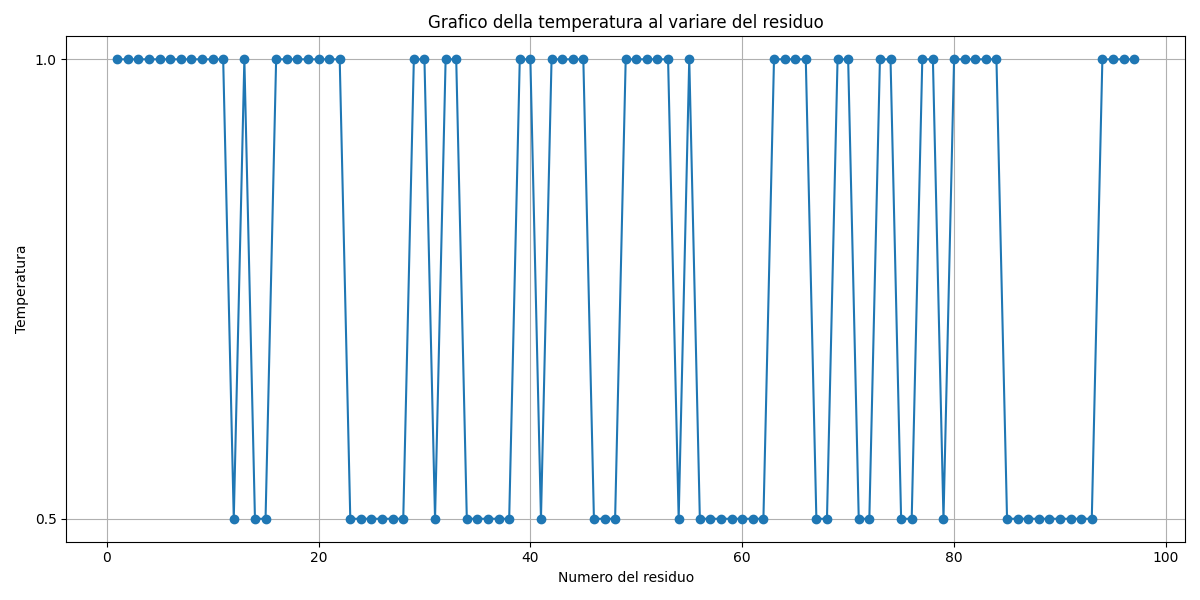
\includegraphics[width=0.5\textwidth]{"images/2m10_2_temperature_cutoff.png"}
    \caption{ Temperatura Troncamento  }
\end{figure}

\section{Temperatura radiale}
T(r)=T_0+(Tb-T0)/R*r

\begin{figure}[H]
    \centering
    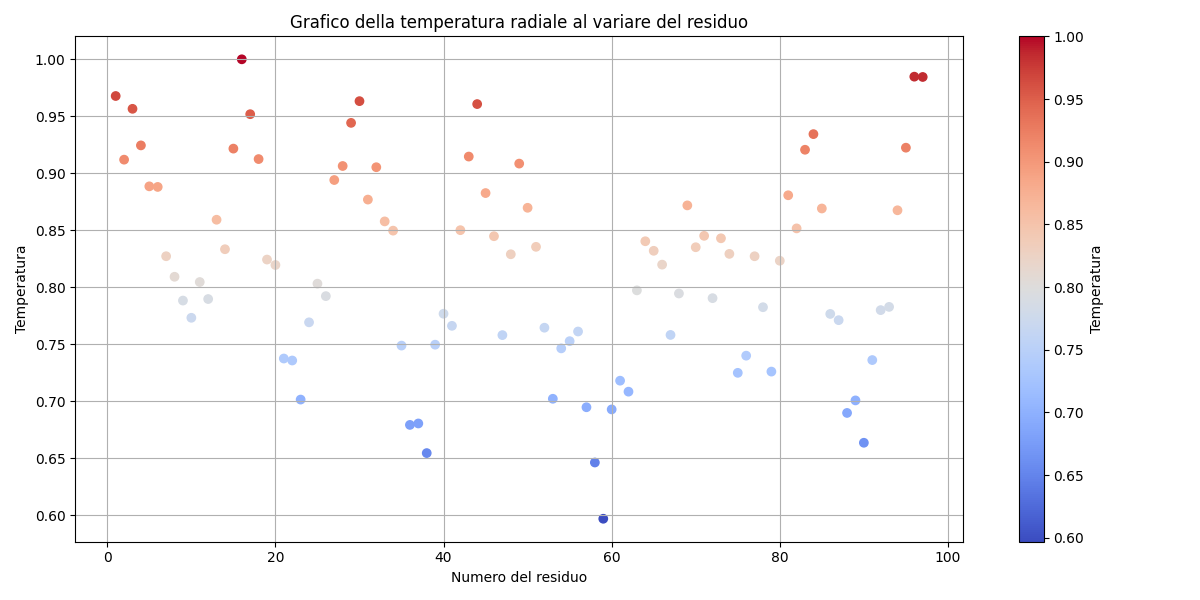
\includegraphics[width=0.5\textwidth]{"images/2m10_2_temperature_sferic.png"}
    \caption{Temperatura Radiale}
\end{figure}
\begin{figure}[H]
    \centering
    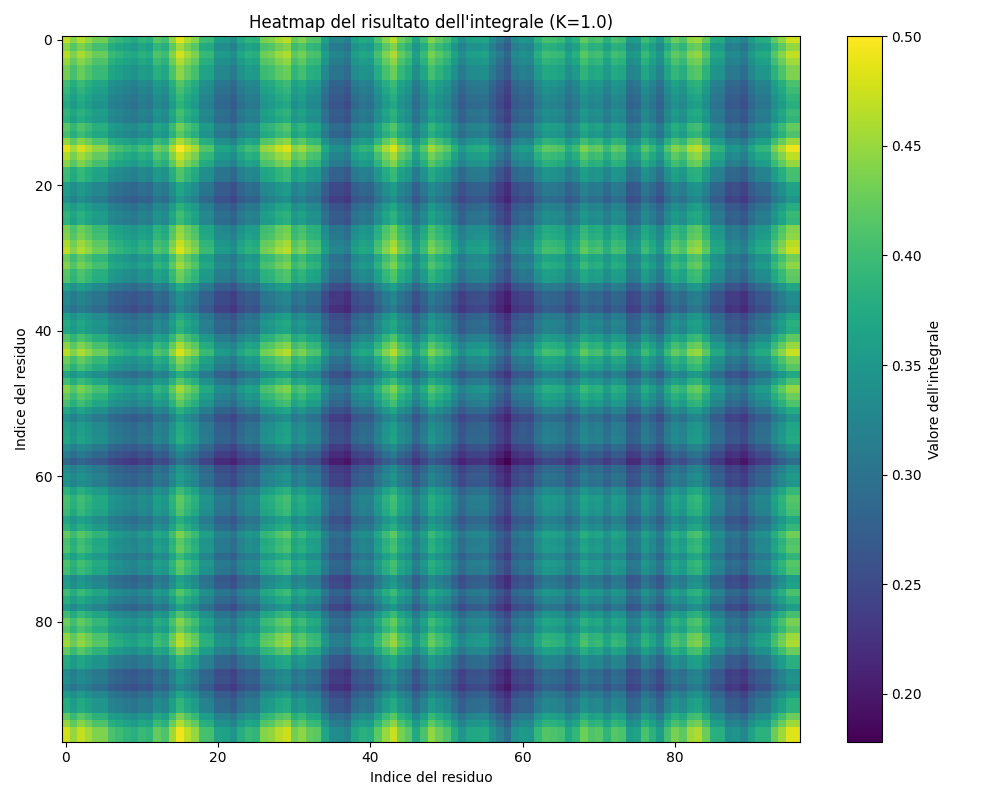
\includegraphics[width=0.5\textwidth]{"images/2m10_2_temperature_correlation_sferic.png"}
    \caption{Correlazione Radiale}
\end{figure}
\end{document}

